\chapter{镜像对称}
现在我们已经定义了与 $A$ 模型和 $B$ 模型相关的 $A_\infty$ 范畴，自然会提出一个问题：
\begin{center}
  \emph{是否能找到某些 $A$ 模型与 $B$ 模型，使它们描述同一个底层 $A_\infty$ 范畴？}
\end{center}
这一现象称为同调镜像对称。若一对 $A$ 模型与 $B$ 模型导出相同的范畴，就称它们为一对镜像。本章将讨论如何寻找可能的镜像对、如何证明它们互为镜像，并说明它们在几何上如何联系。

\section{复环面}\label{sec:complex-torus}
\takeaway{复环面 $T=(\mathbb C^*)^n$ 与 $T^*(S^1)^n$ 互为镜像：wrapped、正合、$\mathbb Z_2$ 分次三种 Fukaya 范畴分别等价于 $D\mathrm{Coh}^{\bullet}$、挠层与矩阵分解。镜像上的点对应底环面 $B$ 上的一维局部系统，因此 $T$ 的镜像是作为对偶群出现的 $T^\vee=\operatorname{Grp}(N,\mathbb C^*)$。}
我们从一个在第\ref{ch:physics-motivation}章已经研究过的例子开始。

\begin{example}[圆柱与复环面的镜像]
考察圆柱
\[
  X=T^*S^1\cong\mathbb C^*,
  \qquad \Omega=\frac{dz}{z},
\]
其中 $\Omega$ 是用于定义分次的体积形式。它可以看作带柱形端的 Liouville 流形。
\begin{itemize}
  \item 相应的 wrapped Fukaya 范畴 $\mathrm{wrFuk}^{\bullet}(X,\Omega)$ 由一个余切纤维生成，其自同态环为集中在次数 $0$ 的
  \[
    R=\mathbb C[X,X^{-1}].
  \]
  因而
  \[
    D^{\infty}\mathrm{wrFuk}^{\bullet}(T^*S^1,\Omega)
    =D^{\infty}R=D\mathrm{Mod}^{\bullet}R.
  \]
  后者与 $D\mathrm{Coh}^{\bullet}Y$ 同构，其中 $Y=V(R)\cong\mathbb C^*$。因此，$(T^*S^1,\mathbb C^*)$ 可以视为一对镜像：
  \[
    D^{\infty}\mathrm{wrFuk}^{\bullet}(T^*S^1,\Omega)
    \cong D\mathrm{Coh}^{\bullet}\mathbb C^*.
  \]
  \item 也可以考察 $T^*S^1$ 的正合 Fukaya 范畴。其对象是带局部系统的紧正合拉格朗日子流形。在同位变形意义下，这样的拉格朗日子流形只有圆周本身；局部系统可看成基本群
  \[
    \pi_1(S^1)=\mathbb Z
  \]
  的有限维表示，或其群环的有限维表示。该群环为
  \[
    \mathbb C[\pi_1(S^1)]\cong\mathbb C[X,X^{-1}]\cong R.
  \]
  于是有等价 $D\mathrm{mod}^{\bullet}R\simeq D\mathrm{Fuk}^{\bullet}X$。从 $B$ 侧看，$R$ 的有限维表示由 $Y=\mathbb C^*$ 上的点层 $S_p$ 生成；这些也称为挠层\index{naoceng@挠层|hyperpage}：
  \[
    D^{\infty}\mathrm{exFuk}^{\bullet}(T^*S^1,\Omega)
    =D^{\infty}\mathrm{tor}^{\bullet}\mathbb C^*
    :=\langle S_p\mid p\in\mathbb C^*\rangle
    \subset D\mathrm{Coh}^{\bullet}\mathbb C^*.
  \]
  \item 最后还可以考察 $\mathbb Z_2$ 分次的 wrapped Fukaya 范畴。它仍由一个余切纤维生成，所以与 $D^{\pm}R$ 等价。在 $B$ 侧，可以把这个范畴实现为矩阵分解范畴
  \[
    \mathrm{MF}^{\pm}(\mathbb C^3,(XY-1)Z).
  \]
  令 $F$ 表示 $\mathbb C[X,Y,Z]$ 上的秩一自由模。上述范畴由对象
  \[
    (F\oplus F,\begin{pmatrix}0&XY-1\\Z&0\end{pmatrix})
  \]
  生成；其自同态环为
  \[
    \mathbb C[X,Y,Z]/(XY-1,Z)\cong\mathbb C[X,X^{-1}]=R.
  \]
  从几何上看，这个 $B$ 模型对应于 $\mathbb C^3$ 中一个超曲面的奇点集；该超曲面由一个二次曲面与一个平面组成，二者的交是一条圆锥曲线，且同构于仿射簇 $\mathbb C^*$。因此
  \[
    D^{\infty}\mathrm{wrFuk}^{\pm}(T^*S^1)
    \simeq\mathrm{MF}^{\pm}(\mathbb C^3,(XY-1)Z).
  \]
\end{itemize}
所以，$\mathbb C^*$ 与 $T^*S^1$ 互为镜像这一事实，体现为三种不同的 $A_\infty$ 范畴等价。
\end{example}

上面的例子可以推广到高维。令
\[
  X=(T^*S^1)^n=T^*(S^1)^n,
  \qquad
  \Omega=\frac{dz_1}{z_1}\wedge\cdots\wedge\frac{dz_n}{z_n}.
\]
wrapped Fukaya 范畴仍由一个余切纤维分裂生成，但其自同态环变为
\[
  \mathbb C[X_1^{\pm1},\ldots,X_n^{\pm1}],
\]
对应的仿射簇为 $(\mathbb C^*)^n$。因此，$(T^*(S^1)^n,(\mathbb C^*)^n)$ 是一对镜像。

底空间 $L=(S^1)^n$ 是 $X$ 中的正合拉格朗日环面。由第\ref{ch:physics-motivation}章可知，给 $L$ 配备平凡局部系统时，其自同态环是环面的上同调环，也就是 $n$ 个变量生成的外代数 $\Lambda_n$。在 $L$ 上选取非平凡局部系统，相当于选择基本群 $\pi_1(L)=\mathbb Z^n$ 的一个表示。这个基本群的群环为
\[
  \mathbb C[X_1^{\pm1},\ldots,X_n^{\pm1}],
\]
故其每个有限维模都给出正合 Fukaya 范畴的一个对象。从 $B$ 侧看，一维简单模对应于
\[
  V\bigl(\mathbb C[X_1^{\pm1},\ldots,X_n^{\pm1}]\bigr)\cong(\mathbb C^*)^n
\]
上的点层。一般而言，坐标环的有限维模所对应的层也称为挠层。无分次版本也可以推广，于是得到下列等价表：
\[
\begin{array}{c|c|c}
\text{$A$ 模型} & \text{代数} & \text{$B$ 模型}\\\hline
D^{\infty}\mathrm{wrFuk}^{\bullet}(T^*(S^1)^n,\Omega)
 &D\mathrm{Mod}^{\bullet}\mathbb C[X_1^{\pm1},\ldots,X_n^{\pm1}]
 &D\mathrm{Coh}^{\bullet}(\mathbb C^*)^n\\
D^{\infty}\mathrm{exFuk}^{\bullet}(T^*(S^1)^n,\Omega)
 &D\mathrm{mod}^{\bullet}\mathbb C[X_1^{\pm1},\ldots,X_n^{\pm1}]
 &D\mathrm{tor}^{\bullet}(\mathbb C^*)^n\\
D^{\infty}\mathrm{wrFuk}^{\pm}(T^*(S^1)^n)
 &D^{\pm}\mathbb C[X_1^{\pm1},\ldots,X_n^{\pm1}]
 &\mathrm{MF}^{\pm}(\mathbb C^{n+2},(X_0\cdots X_n-1)Z)
\end{array}
\]

在上面的例子中，$X=T^*(S^1)^n\cong(\mathbb C^*)^n$ 与 $Y=(\mathbb C^*)^n$ 互为镜像，而 $Y$ 又与 $X$ 同构。这种看法有些迷惑性，因为实际上不应把 $X$ 与 $Y$ 看作同一个空间；它们是对偶的。

乘法群 $(\mathbb C^*)^n$ 称为 $n$ 维复环面，记为 $T$。与之相关的还有两个群：特征群\index{tezhengqun@特征群|hyperpage}
\[
  M:=\operatorname{Grp}(T,\mathbb C^*)
\]
和单参数子群所成的群
\[
  N:=\operatorname{Grp}(\mathbb C^*,T).
\]
二者都同构于 $\mathbb Z^n$。对每个 $u,v\in\mathbb Z^n$，定义
\[
  \chi_u\colon T\to\mathbb C^*,\quad
  (x_1,\ldots,x_n)\longmapsto x_1^{u_1}\cdots x_n^{u_n}\in M,
\]
和
\[
  \lambda_v\colon\mathbb C^*\to T,\quad
  t\longmapsto(t^{v_1},\ldots,t^{v_n})\in N.
\]
这两个群通过自然配对互为对偶：
\[
  \langle u,v\rangle=u_1v_1+\cdots+u_nv_n,
  \qquad \chi_u\circ\lambda_v(t)=t^{\langle u,v\rangle}.
\]
我们可以把 $T$ 重构为 $\operatorname{Grp}(M,\mathbb C^*)$ 或 $V(\mathbb C[M])$，因此定义对偶环面
\[
  T^\vee:=\operatorname{Grp}(N,\mathbb C^*)=V(\mathbb C[N]).
\]
% [Tutor Note: 配对 $\langle u,v\rangle=\sum u_iv_i$ 中 $u\in M$ 是“频率”（出现在单项式指数上），$v\in N$ 是“周期”（单参数子群的生成方向）；$\chi_u\circ\lambda_v(t)=t^{\langle u,v\rangle}$ 说两者相乘才给出数。把 $M,N$ 都识别成 $\mathbb Z^n$ 之后极易把指标写反：本节的射线向量住在 $N$，而对偶锥与势函数的单项式指数住在 $M$。]

回忆一下，$X=T^*(S^1)^n=T$ 的镜像上的点，对应于底空间
\[
  B=\{x\in T\mid|x|=1\}=(S^1)^n
\]
上的一维局部系统；等价地，对应于其基本群的一维表示。这个基本群可以认作 $N$：每个 $\lambda_v$ 都给出一个环路
\[
  \ell_v\colon[0,1]\to B,\qquad
  s\longmapsto\lambda_v(e^{2\pi is}).
\]
因此，$T$ 的镜像自然地可视为
\[
  \operatorname{Hom}(N,\mathbb C^*)=T^\vee.
\]
这一观察将成为我们寻找其他镜像对\index{jingxiangdui@镜像对|hyperpage}的出发点。

\section{环簇}\label{sec:toric-varieties}
\takeaway{环簇由扇（整锥的集合）组合地定义，锥与环面轨道一一对应且 $\dim\sigma=n-\dim O_\sigma$；每个环簇除子 $D_\sigma$ 对应 $B$ 侧势函数中的单项式 $y^{v_\sigma}$，由此猜测 $(X_\Delta,\sum D_\sigma)$ 的镜像是 Landau--Ginzburg 模型 $(T^\vee,W_\hbar)$。}
将镜像对称推广到复环面\index{fuhuanmian@复环面|hyperpage}之外的一种方法，是考察环簇\index{huanzu@环簇|hyperpage}（toric variety）。这类簇以复环面为稠密开子集，并且可以由组合数据定义。环簇理论发展成熟，包含代数几何中许多重要概念的说明性例子。更多内容参见\bookcite{89,57}。

令 $T,T^\vee$ 为上一节中的对偶环面\index{duiouhuanmian@对偶环面|hyperpage}。相应的对偶格记为
\[
  M=\operatorname{Hom}(T,\mathbb C^*)=\operatorname{Hom}(\mathbb C^*,T^\vee),
  \qquad
  N=\operatorname{Hom}(T^\vee,\mathbb C^*)=\operatorname{Hom}(\mathbb C^*,T),
\]
并记 $M_{\mathbb R}=M\otimes_{\mathbb Z}\mathbb R$、$N_{\mathbb R}=N\otimes_{\mathbb Z}\mathbb R$。格与相应实向量空间之间的自然配对记为 $\langle\ ,\ \rangle$。把 $M,N$ 识别为 $\mathbb Z^n$，把 $M_{\mathbb R},N_{\mathbb R}$ 识别为 $\mathbb R^n$，使得该配对就是标准内积。

坐标环 $\mathcal O(T)$ 同构于群环
\[
  \mathbb C[M]=\mathbb C[X_1^{\pm1},\ldots,X_n^{\pm1}].
\]
当 $u\in M=\mathbb Z^n$ 时，把单项式 $X_1^{u_1}\cdots X_n^{u_n}$ 简记为 $X^u$。类似地，
\[
  \mathcal O(T^\vee)=\mathbb C[N]\cong\mathbb C[Y_1^{\pm1},\ldots,Y_n^{\pm1}],
\]
并把与 $v\in N=\mathbb Z^n$ 对应的单项式记作 $Y^v$。

\begin{definition}{整锥}{integral-cone}
$N_{\mathbb R}$ 中的整锥\index{zhengzhui@整锥|hyperpage}是形如
\[
  \sigma=\{\lambda_1v_1+\cdots+\lambda_kv_k\mid
  \lambda_i\in\mathbb R_{\geq0}\}\subset N_{\mathbb R},
  \qquad v_i\in N
\]
的子集。每个锥都有对偶锥\index{duiouzhui@对偶锥|hyperpage}
\[
  \sigma^\vee:=\{u\in M_{\mathbb R}\mid
  \text{对所有 }v\in\sigma,\ \langle u,v\rangle\geq0\}.
\]
对每个 $u\in\sigma^\vee$，还可定义
\[
  \tau_u:=\{v\in\sigma\mid\langle u,v\rangle=0\}.
\]
这些集合仍是整锥，称为 $\sigma$ 的面\index{zhuidemian@锥的面|hyperpage}。
\end{definition}

\begin{definition}{扇}{fan}
扇\index{shan@扇|hyperpage} $\Delta$ 是 $N_{\mathbb R}$ 中整锥构成的集合，并满足：
\begin{itemize}
  \item 若 $\sigma\in\Delta$，且 $\tau$ 是 $\sigma$ 的一个面，则 $\tau\in\Delta$；
  \item 若 $\sigma_1,\sigma_2\in\Delta$，则 $\sigma_1\cap\sigma_2$ 是二者的公共面。
\end{itemize}
$\Delta$ 中所有 $k$ 维锥组成的子集记为 $\Delta_k$。
\end{definition}

扇是一种可用来定义簇的组合数据。每个锥定义群环 $\mathbb C[M]$ 的一个仿射子环
\[
  R_\sigma=\mathbb C[\sigma^\vee\cap M]
  =\mathbb C[X^u\mid u\in\sigma^\vee\cap M],
\]
和仿射簇 $U_\sigma=V(R_\sigma)$。若 $\tau_u$ 是 $\sigma$ 的一个面，则
\[
  \tau_u^\vee=\sigma^\vee+\mathbb R u,
  \qquad R_{\tau_u}=R_\sigma[X^{-u}],
\]
所以 $R_{\tau_u}$ 是 $R_\sigma$ 的局部化。从几何上看，$U_{\tau_u}$ 是 $U_\sigma$ 的开子集。若两个锥 $\sigma_1,\sigma_2$ 有公共面 $\tau$，就可沿图表
\[
  U_{\sigma_1}\longleftarrow U_\tau\longrightarrow U_{\sigma_2}
\]
将它们粘合起来。对扇中的所有锥都这样处理，便得到一个簇。

\begin{definition}{扇所确定的环簇}{toric-variety-from-fan}
簇
\[
  X_\Delta:=\bigcup_{\sigma\in\Delta}U_\sigma
\]
称为与扇 $\Delta$ 对应的环簇。
\end{definition}

\begin{example}[射影平面对应的扇]
令 $N=\mathbb Z^2$，取
\[
  v_1=(1,0),\qquad v_2=(0,1),\qquad v_3=(-1,-1),
\]
并令 $\sigma_i=\mathbb R_{\geq0}v_j+\mathbb R_{\geq0}v_k$，其中 $\{i,j,k\}=\{1,2,3\}$。再令
\[
  \tau_i=\mathbb R_{\geq0}v_i=\sigma_j\cap\sigma_k,
\]
注意 $\sigma_1\cap\sigma_2\cap\sigma_3=\{0\}$。集合
\[
  \Delta=\{\sigma_1,\sigma_2,\sigma_3,\tau_1,\tau_2,\tau_3,\{0\}\}
\]
是一个扇。相应的环为
\[
  R_{\sigma_1}=\mathbb C[YX^{-1},X^{-1}],\quad
  R_{\sigma_2}=\mathbb C[XY^{-1},Y^{-1}],\quad
  R_{\sigma_3}=\mathbb C[X,Y].
\]
这些都是多项式环，所以 $U_{\sigma_i}$ 都同构于 $\mathbb A^2=\mathbb C^2$。它们通过过渡映射粘合；这些映射与射影平面中三个标准仿射平面间的过渡映射一致：
\begin{figure}[H]\centering
  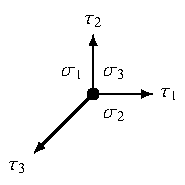
\includegraphics[width=0.37\textwidth]{figures/Fig_125_PDF232_Book220.pdf}
  \caption{射影平面对应的扇（原书 p.220）}
  \label{fig:fan-projective-plane}
\end{figure}
三个仿射片的坐标与齐次坐标之间的变换为
\[
\begin{array}{c|ccc}
 & U_{\sigma_3} & U_{\sigma_2} & U_{\sigma_1} \\ 
X_\Delta & (x,y) & (xy^{-1},y^{-1}) & (yx^{-1},x^{-1}) \\ 
\mathbb P^2 & (x:y:1) & (xy^{-1}:1:y^{-1}) & (1:yx^{-1}:x^{-1})
\end{array}
\]
这些正是射影平面中三个标准仿射片的过渡映射，因此 $X_\Delta\cong\mathbb P^2$。
\end{example}

因为所有环 $R_\sigma$ 都包含在 $\mathbb C[M]$ 中，每个仿射开集 $U_\sigma$ 都包含 $V(\mathbb C[M])=T$。这个开子集是稠密的，并且是群 $G=\mathbb C^{*n}\cong T$ 的一个轨道。$G$ 在各个 $R_\sigma$ 上的作用诱导了 $X_\Delta$ 上的作用，其形式为
\[
  g\cdot X^u=g_1^{u_1}\cdots g_n^{u_n}X^u.
\]
反过来，环簇也可以从这种几何性质刻画。

\begin{theorem}{环簇的扇刻画}{toric-variety-fan-classification}
每个 $n$ 维正规簇 $X$，只要带有 $T=(\mathbb C^*)^n$ 的忠实作用且存在稠密轨道，就来自某个扇 $\Delta$。锥 $\sigma\in\Delta$ 与轨道 $O_\sigma\in X/T$ 一一对应，且
\[
  \dim\sigma=n-\dim O_\sigma.
\]
\end{theorem}
\begin{proof}[证明思路]
固定稠密环面轨道中的一点 $p$。令 $N_+$ 为所有单参数子群\index{dancanshuqun@单参数子群|hyperpage} $\lambda_v\in\operatorname{Grp}(\mathbb C^*,T)$ 所成的集合，其中 $\lim_{t\to0}\lambda_v(t)p$ 在 $X$ 中存在。在 $N_+$ 上定义等价关系：若两个单参数子群给出同一个 $T$-轨道中的极限点，就称它们等价。这个等价关系把 $N_+$ 分成若干等价类 $E$，每个类对应一个轨道。对每个类，取其中向量的所有非负线性组合所成集合的闭包：
\[
  \sigma_E=\overline{\left\{\sum_i\lambda_i v_i\mid
  \lambda_i\in\mathbb R_{\geq0},\ v_i\in E\right\}}.
\]
这些是锥，且全体 $\sigma_E$ 构成所需的扇。为证明 $X_\Delta\cong X$，可构造一个环面等变态射，把 $X_\Delta$ 稠密环面中的一点 $q$ 映到 $p$。由于 $p$ 的轨道在 $X$ 中稠密，该态射是满射；由 $X$ 的正规性可推出它是单射。轨道与锥之间对应关系的更多细节，参见\bookcite[第 3.1 节]{89}。
\end{proof}
% [Tutor Note: “由正规性推出单射”省略的是 Zariski 主定理：正规簇之间的双有理、纤维有限的态射是开浸入；这里轨道分解说明该态射双有理且纤维有限，再加满射即为同构。若 $X$ 不正规，同一个扇给出的映射仍满射，但可能把若干轨道压到同一点，锥与轨道的双射即失效。]

\begin{example}[仿射平面对应的扇]
考察 $\mathbb A^2$，令 $g=(g_1,g_2)\in\mathbb C^*\times\mathbb C^*$ 通过
\[
  g\cdot(x,y)=(g_1x,g_2y)
\]
作用。固定稠密环面 $\mathbb C^*\times\mathbb C^*\subset\mathbb A^2$ 中的点 $(1,1)$。当且仅当 $k_1,k_2\geq0$ 时，极限
\[
  \lim_{t\to0}(t^{k_1},t^{k_2})
\]
存在，因此 $N_+=\mathbb Z_{\geq0}\times\mathbb Z_{\geq0}$。它分成四个等价类：
\[
  \{(0,0)\},\quad \{0\}\times\mathbb Z_{>0},\quad
  \mathbb Z_{>0}\times\{0\},\quad \mathbb Z_{>0}\times\mathbb Z_{>0},
\]
分别对应极限点 $(1,1),(1,0),(0,1),(0,0)$。
\begin{figure}[H]\centering
  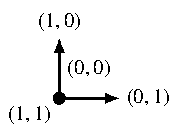
\includegraphics[width=0.25\textwidth]{figures/Fig_126_PDF233_Book221.pdf}
  \caption{仿射平面的扇及轨道极限（原书 p.221）}
  \label{fig:affine-plane-fan-orbits}
\end{figure}
相应的扇为
\[
  \Delta=\{\{(0,0)\},\ \{0\}\times\mathbb R_{\geq0},\
  \mathbb R_{\geq0}\times\{0\},\ \mathbb R_{\geq0}\times\mathbb R_{\geq0}\}.
\]
\end{example}

设 $T=\mathbb C^{*n}$，且 $\pi\colon\widetilde X\to X$ 是环簇之间的满射环面等变态射，并满足 $\pi|_T=1_T$。若两个单参数子群在 $\widetilde X$ 中等价，那么它们在 $X$ 中也等价；因此 $\widetilde X$ 中的锥是 $X$ 中锥的子锥，亦即 $\widetilde X$ 的扇是对 $X$ 的扇作细分所得。反过来，把一个扇细分成更小的锥，会得到一个映到原环簇上的新环簇。

\begin{example}[仿射平面的爆破]
最简单的例子是把仿射平面的锥细分成两个锥：
\begin{figure}[H]\centering
  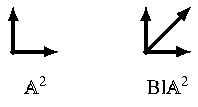
\includegraphics[width=0.36\textwidth]{figures/Fig_127_PDF233_Book221.pdf}
  \caption{$\mathbb A^2$ 的爆破（原书 p.221）}
  \label{fig:blowup-affine-plane-fan}
\end{figure}
在 $\mathbb A^2$ 中，二维锥对应于零轨道。在 $\mathrm{Bl}_0\mathbb A^2$ 中，这个锥被细分为三个锥：两个二维锥各对应一个零维轨道，一个一维锥对应一个一维轨道，该轨道同构于 $\mathbb C^*$。这些轨道合起来构成一条映到原点的 $\mathbb P^1$。换言之，我们把 $\mathbb A^2$ 的原点爆破成一条射影直线。
\end{example}

\begin{example}[$A_{k-1}$ 奇点]\label{ex:ak-singularity-resolution}
考察 $\mathbb R^2$ 中的扇 $\Delta$，其中唯一的二维锥为
\[
  \sigma=\mathbb R_{\geq0}(1,0)+\mathbb R_{\geq0}(1,k).
\]
其对偶锥为
\[
  \sigma^\vee=\mathbb R_{\geq0}(0,1)+\mathbb R_{\geq0}(k,-1),
\]
因此
\[
  \begin{aligned}
  \mathbb C[U_\sigma]
  &=\mathbb C[X^iY^j\mid i\geq0,\ i+kj\geq0]\\
  &=\mathbb C[X^kY^{-1},Y,X]
   \cong\mathbb C[U,V,W]/(UV-W^k).
  \end{aligned}
\]
这个环也是群 $G=\langle g\mid g^k=1\rangle\cong\mathbb Z/k\mathbb Z$ 在 $\mathbb C^2$ 上作用的不变量环，其中
\[
  g(x,y)=(\zeta x,\zeta^{-1}y),
\]
$\zeta$ 是 $k$ 次本原单位根。因此，$X_\Delta$ 同构于仿射商 $\mathbb C^2//G$，而与 $\sigma$ 对应的零维环面轨道就是奇点。

在锥 $\sigma$ 中加入方向为 $v_\ell=(1,\ell)$（$0<\ell<k$）的射线，就可以把 $\sigma$ 细分为 $k$ 个更小的锥。新扇的二维锥为
\[
  \sigma_\ell=\mathbb R_{\geq0}(1,\ell)
  +\mathbb R_{\geq0}(1,\ell+1),\qquad 0\leq\ell<k.
\]
容易验证，对所有 $\ell$，都有 $\mathbb C[U_{\sigma_\ell}]\cong\mathbb C[X,Y]$，所以新的环簇 $\widetilde X$ 是光滑的。
\begin{figure}[H]\centering
  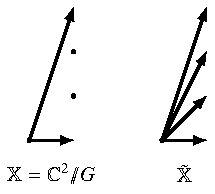
\includegraphics[width=0.54\textwidth]{figures/Fig_128_PDF234_Book222.pdf}
  \caption{$A_{k-1}$ 奇点及其消解（原书 p.222）}
  \label{fig:ak-singularity-resolution}
\end{figure}
每条新增射线给出一个同构于 $\mathbb C^*$ 的环面轨道，每个 $\sigma_\ell$ 给出一个零维环面轨道。它们合起来形成一串 $\mathbb P^1$，在投影映射 $\pi\colon\widetilde X\to X$ 下映到奇点。映射 $\pi$ 称为 $X$ 的一个奇点消解\index{qidianjiexiao@奇点消解|hyperpage}：它是满射、真映射、几乎处处一一对应，并且定义域 $\widetilde X$ 光滑。
\end{example}

前面的定理与例子说明，环簇中的环面轨道与扇的锥一一对应。稠密环面轨道对应零锥，一维锥对应 $(n-1)$ 维轨道。对每个一维锥 $\sigma$，可以定义两个对象：
\begin{itemize}
  \item 射线向量\index{shexianxiangliang@射线向量|hyperpage} $v_\sigma$，即半群 $\sigma\cap N$ 的生成元（最小非零格向量）；
  \item 环簇除子\index{huanzuchuzi@环簇除子|hyperpage} $D_\sigma$，即轨道 $O_\sigma$ 的闭包。
\end{itemize}
后者是一个 $(n-1)$ 维子簇，由所有锥包含 $v_\sigma$ 的轨道组成。由于每个非零锥至少包含一条射线，稠密环面的补集就是所有环簇除子的并：
\[
  X_\Delta\setminus T=\bigcup_{\sigma\in\Delta_1}D_\sigma.
\]

以上观察使我们得以初步猜测环簇的镜像是什么。考虑相对 Fukaya 范畴 $\mathrm{cuFuk}^{\pm}(X_\Delta,D)$，其中
\[
  D=\sum_{\sigma\in\Delta_1}D_\sigma
\]
是所有环簇除子的和。这个范畴是定义在形式幂级数环 $\mathbb C[[\hbar]]$ 上的带曲率形变，其未形变部分是环面 $T$ 的正合 Fukaya 范畴 $\mathrm{exFuk}^{\pm}(T)$。其对象为正合 Fukaya 范畴中的一对 $(L,\rho)$，其中
\[
  L=(S^1)^n\subset\mathbb C^{*n}=T^*(S^1)^n
\]
是拉格朗日基环面，$\rho$ 是基本群
\[
  \pi_1(L)=\pi_1(T)=N
\]
的一个表示。若 $\rho$ 是一维表示，则 $(L,\rho)$ 可认作
\[
  \operatorname{Hom}(N,\mathbb C^*)=T^\vee
\]
中的一点。把该点记作
\[
  (y_1,\ldots,y_n)=(\rho(\ell_1),\ldots,\rho(\ell_n))\in T^\vee,
\]
其中 $\ell_i$ 是 $N=\pi_1(L)=\mathbb Z^n$ 标准基所对应的环路。

将曲率打开，转到相对 Fukaya 范畴时会发生什么？若 $v=v_\sigma$ 是除子 $D_\sigma$ 的射线向量，就可考虑相应的单参数子群
\[
  \lambda_v\colon\mathbb C^*\to T.
\]
由于其在 $t\to0$ 时的极限存在于 $X_\Delta$ 中，$\lambda_v$ 在圆盘 $D\subset\mathbb C$ 上的延拓与限制定义了一张边界落在 $L$ 上、并与 $D_\sigma$ 相交的全纯圆盘。对对象 $(L,\rho)$ 而言，这张全纯圆盘对 $\mu^0$ 的贡献中出现因子
\[
  \rho(\lambda_v|_{S^1})\,\hbar.
\]
其中 $\rho(\lambda_v|_{S^1})$ 来自沿圆盘边界的平行移动，而 $\hbar$ 记录与除子的相交。从镜像一侧看，这意味着每个点 $y=(y_1,\ldots,y_n)\in T^\vee$ 都带有曲率 $W_\hbar(y)$，其中
\[
  W_\hbar=\sum_{\sigma\in\Delta_1}\hbar\,y^{v_\sigma}.
\]
注意，$\mu^0$ 还可能有其他贡献，$\mu^{>0}$ 也可能有贡献；但若运气好，我们找出的这些贡献就足以确定形变的同构类。这提示我们，$(X_\Delta,D)$ 的 $A$ 模型在 $B$ 侧的镜像可能是 Landau--Ginzburg 模型 $(T^\vee,W_\hbar)$。

\begin{note}\label{note:toric-divisor-potential}
\textbf{观察 8.10.} 在 $A$ 模型中加入环簇除子 $D_v$，会在 $B$ 模型的势函数中加入对偶单项式 $y^v$（也可能同时出现其他形变项）。
\end{note}

环簇除子与单项式项的对应关系似乎也可反向使用。回看例\ref{ex:punctured-plane-lg-model}和例\ref{ex:lefschetz-cylinder-quiver}，可见在 $A$ 模型中引入单项式项 $x,x^{-1}$，会得到一个与 $D\mathrm{mod}^{\bullet}\mathbb C Q_3^+$ 等价的有向 Fukaya 范畴。在第\ref{subsec:kronecker-quiver-sheaves}节中我们看到，这与 $\mathbb P^1$ 的导出范畴等价。$\mathbb P^1$ 是一个一维环簇，对应于扇
\[
  \Delta=\{0,\mathbb R_{\geq0},\mathbb R_{\leq0},\mathbb R\},
\]
其两个环簇除子为 $D_{+1}=\{0\}$、$D_{-1}=\{\infty\}$，相应的射线向量为 $N$ 中的 $\pm1$。

\begin{figure}[H]\centering
  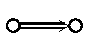
\includegraphics[width=0.33\textwidth]{figures/Fig_129_PDF235_Book223.pdf}
  \caption{有向 Fukaya 范畴中的两个生成对象（原书 p.223）}
  \label{fig:two-arrow-quiver}
\end{figure}
上图中的两个对象与 $\mathbb P^1$ 的两个环簇除子相对应。其扇由一维格 $N\cong\mathbb Z$ 中的两条射线及其交集构成：
\begin{figure}[H]\centering
  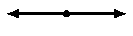
\includegraphics[width=0.22\textwidth]{figures/Fig_130_PDF235_Book223.pdf}
  \caption{$\mathbb P^1$ 的扇（原书 p.223）}
  \label{fig:fan-projective-line}
\end{figure}

\begin{note}\label{note:monomial-toric-divisor}
\textbf{观察 8.11.} 在 $A$ 模型的势函数中加入单项式项 $y^v$，对应于在 $B$ 模型中引入环簇除子 $D_v$。
\end{note}

请注意，目前这些观察还只是一些猜想性的提示，说明 $A$ 模型与 $B$ 模型之间可能如何关联。要得到更精确的结论，我们还需要引入另一种几何。

\section{热带几何}\label{sec:tropical-geometry}
\takeaway{令 $t\to\infty$，超曲面 $W_t^{-1}(0)$ 的阿米巴收缩为热带超曲面 $H_{\mathrm{trop}}$，后者是分段线性函数 $W_{\mathrm{trop}}=\max_m\lambda_m$ 不光滑的轨迹；热带曲线的腿数与亏格分别等于 Newton 多边形的边界格点数与内部格点数，并给出 $\square$ 的对偶三角剖分。}
Landau--Ginzburg 模型由一个带全纯函数的簇 $(Y,W)$ 构成。正如上一节所见，我们尤其关心簇为对偶环面 $T^\vee$、且势函数
\[
  W_\hbar\colon T^\vee\to\mathbb C
\]
依赖形变参数 $\hbar$ 的情形。一般而言，$A$ 模型 $(Y,W)$ 并不依赖 $\hbar$；因此我们将考察 $\hbar\to0$ 时的情形，或者等价地，令参数 $t=\hbar^{-1}$ 趋于无穷。这会引出一种称为热带几何的新几何。该领域的综述可参见 Mikhalkin\bookcite{175}，入门专著可参见 Maclagan 与 Sturmfels\bookcite{181}。

考虑一族 Laurent 多项式
\[
  W_t\in\mathbb C[Y_1^{\pm1},\ldots,Y_n^{\pm1},t^{\pm1}],
\]
并考察给定 $t\in\mathbb R_{>0}$ 时，对偶环面 $T^\vee$ 中由 $W_t$ 定义的超曲面。这类超曲面的拓扑不总是容易可视化，但可以通过阿米巴\index{amiba@阿米巴|hyperpage}来研究。\footnote{阿米巴（amoeba，源自希腊语“变形虫”）是复环面中超曲面在逐坐标对数映射下的像；它通常呈一只带腿的厚实变形虫之形，故得名。这一概念由 Gelfand、Kapranov 与 Zelevinsky 引入\bookcite{106}，其后在热带几何的研究中得到发展\bookcite{86,175}。}

\begin{definition}{Gelfand--Zelevinsky--Kapranov\bookcite{106}}{rescaled-amoeba}
定义映射
\[
  \log_t\colon T^\vee\to\mathbb R^n,
  \qquad (y_1,\ldots,y_n)\longmapsto
  \frac{1}{\ln|t|}(\ln|y_1|,\ldots,\ln|y_n|).
\]
$W_t$ 的（缩放）阿米巴是 $W_t^{-1}(0)$ 在此对数映射下的像：
\[
  A_t:=\log_t\{(y_1,\ldots,y_n)\in\mathbb C^{*n}\mid
  W_t(y_1,\ldots,y_n)=0\}.
\]
\end{definition}

\begin{example}[一个 Laurent 多项式的阿米巴]
取 $t=2$，令
\[
  W_t=X^2Y^3+X^2Y^2+tX^2Y-5XY^2+3XY-Y^2+t^2Y+1.
\]
它的阿米巴是由下图中的弯曲曲线围成的区域。
\begin{figure}[H]\centering
  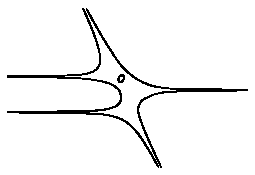
\includegraphics[width=0.53\textwidth]{figures/Fig_131_PDF236_Book224.pdf}
  \caption{例 8.13 中 Laurent 多项式的阿米巴（原书 p.224）}
  \label{fig:amoeba-example-813}
\end{figure}
\end{example}

一般而言，$\mathbb C^{*2}$ 中超曲面的阿米巴看起来像一张加厚的分段线性图，带有若干条无限延伸的腿。令 $t$ 趋于无穷时，这层加厚会逐渐收缩，极限就是那张图。

为精确说明这一点，把
\[
  W_t=\sum_{m\in M}c_m t^{k_m}Y^m
\]
写成单项式之和，其中指数 $m\in M\subset\mathbb Z^n$，系数由 $c_m\in\mathbb C^*$ 与 $t$ 的整数次幂 $k_m\in\mathbb Z$ 构成。令 $t$ 趋于无穷时，阿米巴 $A_t$ 趋近某个多面体骨架。原因是当 $t$ 很大时，在大多数点上，$W_t(y)$ 的某个单项式会占主导，因此 $W_t(y)\ne0$。只有当两个单项式大小相等时，它们才可能相消而使总和为零。每个单项式 $c_mt^{k_m}Y^m$ 定义线性函数
\[
  \lambda_m\colon\mathbb R^n\to\mathbb R,
  \qquad u\longmapsto\langle u,m\rangle+k_m.
\]
因此，$A_t$ 中的点集中在最大值同时由至少两个函数 $\lambda_m$ 取得的位置附近。

\begin{definition}{热带函数与热带超曲面}{tropical-function-hypersurface}
设 $W_t=\sum_{m\in M}c_mt^{k_m}Y^m$，其对应的热带函数\index{redaihanshu@热带函数|hyperpage}为
\[
  W_{\mathrm{trop}}\colon\mathbb R^n\to\mathbb R,
  \qquad u\longmapsto\max_{m\in M}\lambda_m(u).
\]
它是 $\mathbb R^n$ 上的分段线性函数，并把 $\mathbb R^n$ 分成若干胞腔 $\overline B_m$；在 $\overline B_m$ 上，$W_{\mathrm{trop}}$ 等于与单项式 $m$ 对应的线性函数 $\lambda_m$。热带超曲面\index{redaichaoqumian@热带超曲面|hyperpage} $H_{\mathrm{trop}}$ 是 $W_{\mathrm{trop}}$ 不光滑的轨迹；等价地，它是 $W_{\mathrm{trop}}$ 的最大值由多个线性函数同时取得的点集。换言之，它是所有 $\overline B_m$ 的内部之补集。
\end{definition}

\begin{theorem}{阿米巴的热带极限\bookcite{175,86}}{amoeba-tropical-limit}
设 $W_t\in\mathbb C[Y_1^{\pm1},\ldots,Y_n^{\pm1},t^{\pm1}]$ 是 Laurent 多项式。当 $t\in\mathbb C^*$ 趋于无穷时，阿米巴 $A_t$ 趋近热带超曲面 $H_{\mathrm{trop}}$。特别地，当 $|t|$ 足够大时，$\mathbb R^n\setminus A_t$ 由若干区域 $(B_m)_t$ 组成；每个区域对应于 $W_t$ 中某个单项式 $c_mt^{k_m}Y^m$ 占主导的位置。在极限下，$(B_m)_t$ 变为凸多面体胞腔 $\overline B_m$，此处相应的线性函数 $\lambda_m$ 在 $W_{\mathrm{trop}}$ 中占主导。
\end{theorem}
% [Tutor Note: “阿米巴 $A_t$ 趋近 $H_{\mathrm{trop}}$”的严格含义是：对任意紧集 $K$，$A_t\cap K$ 与 $H_{\mathrm{trop}}\cap K$ 的 Hausdorff 距离当 $|t|\to\infty$ 时趋于零。证明的关键只是初等估计——系数 $t^{k_m}$ 增长最快的单项式在远离折点处严格支配其余项，故交点只能出现在两个指数并列最大的位置。]

胞腔 $\overline B_m$ 是凸的，其边界由形如
\[
  \lambda_{m_1}(u)-\lambda_{m_2}(u)=0
\]
的超平面组成。这些超平面的交叠可能相当复杂，因此常常需要施加一般性条件。

\begin{definition}{Newton 多面体与通有热带函数\index{tongyouredaihanshu@通有热带函数|hyperpage}}{generic-tropical-function}
$W_{\mathrm{trop}}$ 的 Newton 多面体\index{newtonduomianti@Newton 多面体|hyperpage} $\square$ 是 $M\subset\mathbb Z^n$ 在 $\mathbb R^n$ 中的凸包。若对每个格点 $m\in\square\cap\mathbb Z^n$，胞腔 $\overline B_m$ 都有非空内部，且各超平面 $\lambda_{m_1}(u)-\lambda_{m_2}(u)=0$ 均横截相交，则称 $W_{\mathrm{trop}}$ 是通有的。
\end{definition}

下面集中讨论通有热带曲线\index{tongyou@通有|hyperpage}，即 $n=2$ 的情形。此时 Newton 多面体是一个多边形，热带曲线是嵌入 $\mathbb R^2$ 的图，其中有有限边和无限边；无限边称为腿。我们把单项式分成两类：指数位于 Newton 多边形内部的单项式，与指数位于边界上的单项式。分别记这两类指数集合为 $I$ 与 $B$。若 $m$ 是内部格点，则 $\overline B_m$ 是有界凸多边形；若 $m$ 是边界格点，则 $\overline B_m$ 是被两条趋向无穷远的热带曲线之腿夹住的无界区域。因此，热带曲线的无限腿总数为 $\#B$，其紧部分中的孔洞数为 $\#I$。

在通有情形下，图的顶点都是三价的，因为若某顶点价数更高，就意味着多于三个线性函数 $\lambda_i\colon\mathbb R^2\to\mathbb R$ 在同一点取相同值，这与横截相交条件矛盾。于是对每个顶点 $v\in H_{\mathrm{trop}}$，可以在多边形 $\square$ 中画一个小三角形\index{jibensanjiaoxing@基本三角形|hyperpage}，连接那些对应区域在 $v$ 处相邻的格点。这样便得到一个与 $H_{\mathrm{trop}}$ 对偶的三角剖分。每个三角形恰含三个格点，且都位于顶点处；这样的三角形称为基本三角形。

由于 $t$ 足够大时 $A_t$ 趋近 $H_{\mathrm{trop}}$，曲线
\[
  \dot S:=W_t^{-1}(0)\subset T^\vee
\]
可看作一条绕着 $H_{\mathrm{trop}}$ 延展、带有若干穿孔的黎曼曲面。因此，该曲面的亏格为 $\#I$，穿孔数为 $\#B$。沿热带曲线的有限边切开曲面，可将其分解为若干个裤子曲面。

\begin{example}[亏格为一的热带曲线]
取函数
\[
  W_t=t^8+tX^{-1}Y^{-1}+t^2Y^{-1}+tXY^{-1}+t^4Y.
\]
其热带函数为
\[
  W_{\mathrm{trop}}=\max\{8,\,1-X-Y,\,2-Y,\,1+X-Y,\,4+Y\}.
\]
热带曲线及 Newton 多边形的相应三角剖分如下图所示。
\begin{figure}[H]\centering
  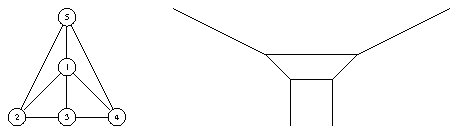
\includegraphics[width=0.66\textwidth]{figures/Fig_132_PDF238_Book226.pdf}
  \caption{例 8.17 的热带曲线与 Newton 多边形三角剖分（原书 p.226）}
  \label{fig:tropical-curve-genus-one}
\end{figure}
因此，对通有的 $t$，曲面 $\dot S=W_t^{-1}(0)\subset\mathbb C^{*2}$ 的亏格为 $1$，并有四个穿孔。
\end{example}

\section{一、二、三维镜像对称}\label{sec:one-two-three-mirror-symmetry}
\takeaway{同一个二维 Newton 多边形 $\square$ 可在复维 $1,2,3$ 中构造镜像：$A$ 侧依次是带穿孔黎曼曲面、Landau--Ginzburg 模型以及由 $UV=W_t$ 切出的三维超曲面；$B$ 侧是仿射环簇及其环簇除子，对应关系由矩阵分解、凝聚层与 wrapped/有向/正合 Fukaya 范畴的分裂导出等价给出。}
现在我们将研究镜像对称与环簇几何、热带几何之间的关系。出发点是 $n$ 维复环面上的一参数函数族
\[
  W_t\colon T^\vee\to\mathbb C,
\]
它使我们可以探索 $n-1,n,n+1$ 维中的镜像对称。为简单起见，假设 $\dim T^\vee=2$，于是得到一、二、三维中的对应关系。

\subsection{模型}\label{subsec:one-two-three-models}
我们先定义三个 $A$ 模型。每种情形中的辛几何都不依赖参数 $t$，因此可以令 $t\to\infty$，考察热带极限。于是 $A$ 模型只依赖于 Newton 多边形；当 $n=2$ 时，它是一个多边形。将其记为 $\square$，并用它作为以下三个 $A$ 模型的下标：
\begin{itemize}
  \item[(1D)] $Y^1_\square:=W_t^{-1}(0)$ 是对偶环面 $T^\vee=(\mathbb C^*)^2$ 中带穿孔的黎曼曲面。把穿孔附近补成柱形端后，它可视为一个 Liouville 子流形。
  \item[(2D)] $Y^2_\square:=(T^\vee,W_t)$ 是定义在复环面 $T^\vee\cong T^*(S^1)^2$ 上的 Landau--Ginzburg 模型，配备标准正合辛结构与体积形式。
  \item[(3D)]
  \[
    Y^3_\square:=\{(X,Y,U,V)\in T^\vee\times\mathbb C^2\mid
      UV=W_t(X,Y)\}
  \]
  是一个超曲面，可视为 $T^\vee\times\mathbb C^2=T^*(S^1)^2\times\mathbb R^2$ 中的正合辛子流形。也可以把它看作 $T^\vee$ 上的仿射圆锥截面族；当 $W_t=0$ 时，圆锥截面退化。
\end{itemize}
% [Tutor Note: 三个模型名字里的 1D、2D、3D 指复维数：$Y^1_\square$ 是黎曼曲面（实维 2），$Y^2_\square=(T^\vee,W_t)$ 是复曲面上的 Landau--Ginzburg 模型（实维 4），而 $Y^3_\square$ 是 $T^\vee\times\mathbb C^2$ 中由一个方程切出的超曲面，实维为 $4+4-2=6$。写镜像对应时不要混用复维与实维。]

由于 $W_t$ 是对偶环面 $T^\vee$ 上的函数，它的单项式指数属于 $N=\operatorname{Hom}(T^\vee,\mathbb C^*)$，所以 Newton 多边形是 $N_{\mathbb R}$ 的子集。在通有情形下取极限时，热带函数 $W_{\mathrm{trop}}$ 会在 Newton 多边形上诱导一个三角剖分，记作 $\boxtimes$。这个三角剖分将用于构造三个 $B$ 模型。

\begin{itemize}
  \item[(3D)] 把 Newton 多边形放在三维空间中的高度 $1$ 平面
  \[
    \square\times\{1\}\subset\mathbb R^3
  \]
  上，取它所张成的锥
  \[
    \sigma_\square=\mathbb R_{\geq0}(\square\times\{1\}).
  \]
  这确定一个三维仿射环簇
  \[
    X^3_\square=V(\mathbb C[\sigma_\square^\vee\cap M]).
  \]
  除非 $\square$ 是基本三角形（此时 $X^3_{\triangle}\cong\mathbb A^3$），否则该簇是奇异的。仿照例\ref{ex:ak-singularity-resolution}，把这个锥细分为覆盖三角剖分 $\boxtimes$ 中各基本三角形的小锥，即可消解奇点。这样得到光滑的三维环簇 $X^3_{\boxtimes}$ 和消解映射
  \[
    \pi\colon X^3_{\boxtimes}\to X^3_\square.
  \]
  这种消解称为 crepant 消解\index{crepantxiaojie@crepant 消解|hyperpage}。\footnote{消解 $\widetilde X\to X$ 称为 crepant 的，若 $X$ 上典范线丛的拉回等于 $\widetilde X$ 上的典范线丛。}
  % [Tutor Note: 环簇情形下“crepant”有一个纯组合的判据：细分所用的每条新射线都落在原锥的高度 $1$ 截面上（这里就是 $\square$ 的格点 $(a,b,1)$），于是细分不引入新的典范除子，$K_{X^3_\boxtimes}=\pi^*K_{X^3_\square}$。若射线来自更高层（如 $(a,b,2)$ 方向），消解就会多出未被消去的除子。]
  \begin{figure}[H]\centering
    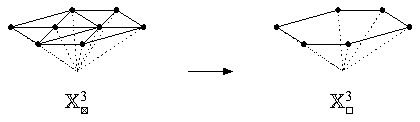
\includegraphics[width=0.73\textwidth]{figures/Fig_133_PDF240_Book228.pdf}
    \caption{三维仿射环簇及其消解（原书 p.228）}
    \label{fig:toric-threefold-crepant-resolution}
  \end{figure}
  \item[(2D)] $X^3_{\boxtimes}$ 的射线向量形如 $v=(a,b,1)$，其中 $(a,b)$ 是 Newton 多边形中的格点。令 $m=(0,0,1)$，则对所有射线向量 $v$ 都有 $\langle m,v\rangle=1$。这意味着函数
  \[
    \ell=X^m
  \]
  属于所有 $\mathcal O(U_\sigma)$，因此是一个整体函数。它的零点集是稠密环面的补集
  \[
    D=X^3_{\boxtimes}\setminus T,
  \]
  也就是所有环簇除子 $D_v$ 的并。每个环簇除子 $D_v$ 本身也是光滑环簇。其扇可如下构造：若射线向量 $v,w_1,w_2$ 构成 $\boxtimes$ 中的一个基本三角形，则
  \[
    \mathbb R_{\geq0}(w_1-v)+\mathbb R_{\geq0}(w_2-v)
  \]
  是平面 $\mathbb R^2\times\{0\}$ 中的一个锥。若 $v$ 是 $\square$ 的内部格点，该扇覆盖整个 $\mathbb R^2$，且 $D_v$ 位于消解映射 $\pi\colon X^3_{\boxtimes}\to X^3_\square$ 的零纤维中。我们把这个除子记为 $X^2_v$。
  \begin{figure}[H]\centering
    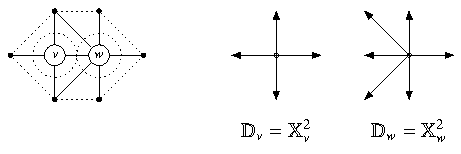
\includegraphics[width=0.55\textwidth]{figures/Fig_134_PDF240_Book228.pdf}
    \caption{环簇除子的局部扇（原书 p.228）}
    \label{fig:toric-divisor-fans}
  \end{figure}
  \item[(1D)] 最后考察 Landau--Ginzburg 模型
  \[
    X^1_{\boxtimes}:=(X^3_{\boxtimes},\ell).
  \]
  从 $B$ 模型的角度，它描述 $\ell$ 的零点集中的奇点；该奇点集是一维的。正如我们已经看到的，$\ell^{-1}(0)=X^2_{\boxtimes}$ 是若干光滑环簇除子的并，其奇点集就是这些除子的交。若 $D_v,D_w$ 的射线向量在扇中张成二维锥，那么这两个除子有一个公共的一维环面轨道（即 $\mathbb C^*$）。这恰好意味着三角剖分中的相应格点以一条边相连。若三个除子相交于一点，则其射线向量张成三维锥，也就是说相应三个格点构成三角剖分中的一个三角形。
\end{itemize}

因此，我们可以把具有同一三角剖分的热带曲线的几何与 $\ell^{-1}(0)$ 的奇点集联系起来。$\ell^{-1}(0)$ 的奇点集在热带曲线的每条边上有一个 $\mathbb C^*$，在每个顶点上有一个点。每条内部边连接两个顶点，相应的两个点与 $\mathbb C^*$ 合起来构成一个 $\mathbb P^1$；每条腿只连接一个顶点，所以相应的点与 $\mathbb C^*$ 合起来构成一个 $\mathbb A^1$。故奇点集是若干条射影直线与仿射直线组成的并，它们在三重交点处相接。
\begin{figure}[H]\centering
  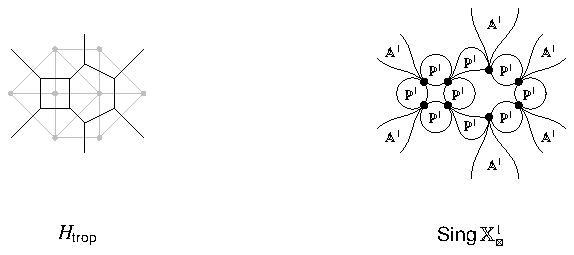
\includegraphics[width=0.92\textwidth]{figures/Fig_135_PDF241_Book229.pdf}
  \caption{热带曲线及 $X^1_{\boxtimes}$ 的奇点集（原书 p.229）}
  \label{fig:tropical-curve-singularity-locus}
\end{figure}

现在可以陈述三维中的镜像对应关系：
\begin{itemize}
  \item[(1D)] Landau--Ginzburg 模型 $X^1_{\boxtimes}$ 的矩阵分解范畴与带穿孔黎曼曲面 $Y^1_\square$ 的 wrapped Fukaya 范畴分裂导出等价：
  \[
    D^\pi\mathrm{MF}^{\pm}X^1_{\boxtimes}
    \simeq D^\pi\mathrm{wrFuk}^{\pm}Y^1_\square.
  \]
  \item[(2D)] 对 Newton 多边形中的每个内部格点 $v$，除子 $X^2_v$ 的凝聚层导出范畴嵌入 $Y^2_\square$ 这一 Landau--Ginzburg 模型的有向 Fukaya 范畴的分裂导出范畴：
  \[
    D\mathrm{Coh}^{\bullet}X^2_v
    \hookrightarrow D^\pi\mathrm{drFuk}^{\bullet}Y^2_\square.
  \]
  若 $X^2_v=\ell^{-1}(0)$，则这个嵌入是等价。
  \item[(3D)] 支撑在 $X^2_v$ 上的 $X^3_{\boxtimes}$ 凝聚层导出范畴嵌入 $Y^3_\square$ 的正合 Fukaya 范畴的分裂导出范畴：
  \[
    D\mathrm{Coh}^{\bullet}_{X^2_v}(X^3_{\boxtimes})
    \hookrightarrow D^\pi\mathrm{exFuk}^{\bullet}Y^3_\square.
  \]
\end{itemize}
构造这些等价有多种方法。下面简要说明每个维数中解决问题的思路。

\subsection{一维情形}\label{subsec:hms-dimension-one}
第一种方法是在两侧分别找出一组分裂生成元，再证明它们的 $A_\infty$ 自同态代数 $A_\infty$ 同构。一维情形的例子见\bookcite{1}。该文作者先考虑 Newton 多边形为基本三角形的情形。此时 $A$ 模型是三穿孔球面
\[
  Y^1_{\triangle}=\{(x,y)\in\mathbb C^{*2}\mid x+y+1=0\}
  \cong\mathbb C^*\setminus\{-1\},
\]
把穿孔补为柱形端后便是裤子曲面。$B$ 模型是 Landau--Ginzburg 模型
\[
  X^1_{\triangle}=(\mathbb A^3,XYZ),
\]
其奇点集由三条坐标轴组成。

$Y^1_{\triangle}$ 的 wrapped Fukaya 范畴有一组简单的锥形拉格朗日子流形 $L_x,L_y,L_z$，它们是分别连接两条柱形端的三条曲线。这些曲线把球面切成两个三角形，因此分裂生成 Fukaya 范畴。矩阵分解范畴也有三个简单的分裂生成元，它们对应于 $\mathbb A^3$ 中三条坐标轴的矩阵分解：
\[
  M_X=\left(R\underset{YZ}{\overset{X}{\rightleftarrows}}R\right),
  \quad M_Y=\left(R\underset{XZ}{\overset{Y}{\rightleftarrows}}R\right),
  \quad M_Z=\left(R\underset{XY}{\overset{Z}{\rightleftarrows}}R\right).
\]
\begin{figure}[H]\centering
  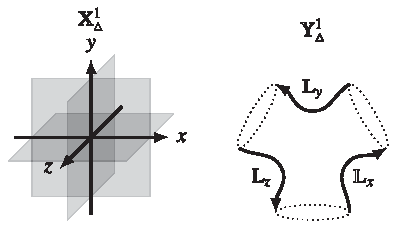
\includegraphics[width=0.92\textwidth]{figures/Fig_136_PDF242_Book230.pdf}
  \caption{裤子曲面上的三个生成曲线（原书 p.230）}
  \label{fig:pants-three-generators}
\end{figure}
\begin{figure}[H]\centering
  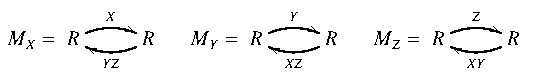
\includegraphics[width=0.88\textwidth]{figures/Fig_137_PDF242_Book230.pdf}
  \caption{三个坐标轴对应的矩阵分解（原书 p.230）}
  \label{fig:coordinate-axis-matrix-factorizations}
\end{figure}
可以计算出，两组生成元的 $A_\infty$ 自同态代数彼此 $A_\infty$ 同构，因此它们分裂生成的范畴等价。更多细节见第~\ref{sec:gentle-algebra-deformations}~节（参见定理~\ref{thm:gentle-ainfty-classification}）。

\begin{note}\label{note:pants-mirror-extensions}
\textbf{注 8.18.} Abouzaid 等人\bookcite{1}通过考察裤子曲面的覆盖，把这一技巧推广到更高亏格、带更多穿孔的黎曼曲面。在 $B$ 侧，这会得到一个带栈结构的 Landau--Ginzburg 模型；该模型也等价于一个拟射影模型。在文献\bookcite{36}中，同一技巧被用于构造非交换镜像，再利用箭图模空间将它们转化为拟射影模型。Pascaleff 与 Sibilla\bookcite{204}、Lee\bookcite{155}还发展了另一种方法：把三穿孔球面对应关系当作基本构件来处理其他情形。此时不寻找生成元，而是把多个三穿孔球面的 $A_\infty$ 范畴粘合起来。在 $A$ 侧，这种粘合可解释为把圆柱管缝在一起；在 $B$ 侧，则可看成把环境空间变为环簇。第\ref{ch:gluing}章将更详细地讨论这一点。最后，Nadler 与 Gammage\bookcite{190,94}提出的另一种粘合方法，把裤子曲面及其他带穿孔曲面的 Fukaya 范畴与微局部层理论联系起来。
\end{note}

\subsection{二维情形}\label{subsec:hms-dimension-two}
二维情形中的 $A$ 模型是一个 Landau--Ginzburg 模型。其对象是 $T^\vee$ 中边界落在 $W_t^{-1}(0)=Y^1_\square$ 上的拉格朗日圆盘。$Y^1_\square$ 在映射 $\log_t\colon T^\vee\to\mathbb R^2$ 下的像是 $W_t=\sum_{w\in\square}t^{a_w}Y^w$ 的阿米巴，是一块带若干孔的区域，这些孔记作 $(B_v)_t$。在通有情形下，每个孔对应 Newton 多边形中的一个格点 $v\in\square$。当 $t\to\infty$ 时，对应于 $v$ 的孔趋近多边形区域
\[
  \overline B_v=\{u\in\mathbb R^2\mid
  \text{对所有使 }[v,w]\text{ 成为 }\boxtimes\text{ 中一条边的 }w,
  \ \langle w-v,u\rangle+a_w-a_v\leq0\}.
\]
注意，向量 $w-v$ 正是 $X^2_v$ 的射线向量。为得到二维对应关系（更高维同理），Abouzaid\bookcite{5}比较了 $X^2_v$ 上的线丛与拉格朗日圆盘；当 $t\to\infty$ 时，这些圆盘经 $\log_t$ 映到 $(B_v)_t$ 上。

若 $X_\Delta$ 是环簇，且 $d\colon S_\Delta:=\Delta_1\to\mathbb Z$ 是从射线向量集合到整数的映射，则可在 $X_\Delta$ 上定义凝聚层 $\mathcal O(d)$：
\[
  \mathcal O(d)(U_\sigma)
  =\mathbb C\{X^m\mid\text{对所有 }v\in S_\Delta\cap\sigma,
    \ \langle v,m\rangle+d_v\geq0\}.
\]
从定义可见，$\mathcal O(0)=\mathcal O$ 是 $X_\Delta$ 的结构层；对每个 $d$，$\mathcal O(d)(U_\sigma)$ 都是有限生成的 $\mathcal O(U_\sigma)$-模。若 $X$ 光滑，则可证明对每个锥 $\sigma$，$\mathcal O(d)(U_\sigma)$ 都是秩一自由模，所以 $\mathcal O(d)$ 是线丛。其整体截面由多边形
\[
  P_d=\{m\in M_{\mathbb R}\mid
  \text{对所有 }v\in S_\Delta,\ \langle v,m\rangle+d_v\geq0\}
\]
中格点对应的单项式张成。
% [Tutor Note: 原文用 $S_\Delta$ 表示射线向量的集合，而前文（例 8.5 之后）把一维锥的集合记作 $\Delta_1$，二者应是同一个集合，属于记号不统一（见原书 p.231）。又 $\mathcal O(d)$ 的数据是每条射线上的整数 $d_v$，故 $d$ 的自由度就是射线数，在二维时等于 Newton 多边形的边数。]

若所有 $d_v$ 均为正，$P_d$ 与 $\overline B_v$“形状相同”（更准确地说，边的法向量方向相反）。因此存在一个光滑映射
\[
  \phi\colon\overline B_v\to P_d
\]
把角点对应起来，如下图所示。
\begin{figure}[H]\centering
  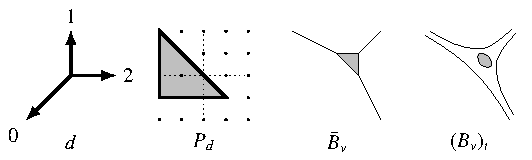
\includegraphics[width=0.86\textwidth]{figures/Fig_138_PDF244_Book232.pdf}
  \caption{线丛多边形与热带胞腔的对应（原书 p.232）}
  \label{fig:line-bundle-polytope-tropical-cell}
\end{figure}

把 $T^\vee$ 分解为
\[
  T^\vee\cong(S^1)^2\times\mathbb R^2=M_{\mathbb R}/M\times\mathbb R^2,
\]
并构造映射
\[
  \widetilde\phi\colon\overline B_v\to T^\vee,
  \qquad u\longmapsto(\phi(u)+M,u).
\]
它把 $\overline B_v$ 缠绕在实环面上，并且是 $\log_t|_{\overline B_v}$ 的截面。当 $t$ 足够大时，区域 $(B_v)_t$ 与 $\overline B_v$ 足够接近，可以微调这个映射，得到 $\log_t|_{(B_v)_t}$ 的一个拉格朗日截面 $L_d$，且它的边界落在 $W_t^{-1}(0)$ 上。这是 $Y^2_{\boxtimes}$ 的有向 Fukaya 范畴中的对象。

在特殊情形 $d=0$ 时，多边形 $P_d$ 是原点，$\phi$ 是常值映射；它提升为常值截面 $L_0$。$L_0$ 与 $L_d$ 的交点对应于 $P_d$ 中的格点，这正符合 $L_0,L_d$ 分别对应线丛 $\mathcal O(0),\mathcal O(d)$ 的预期。在文献\bookcite{5}中，Abouzaid 构造了 $X^2_{\boxtimes,v}$ 上的线丛预范畴到 $Y^2_{\boxtimes}$ 有向 Fukaya 预范畴中的嵌入。

对环簇而言，这些线丛分裂生成凝聚层的整个导出范畴\bookcite[命题 1.3]{5}。在 Fukaya 一侧，可以证明所有紧致 $(B_v)_t$ 上方的拉格朗日截面生成有向 Fukaya 范畴。因此，当内部格点只有一个时，该嵌入诱导导出等价。Abouzaid\bookcite{5}在所有维数中详细构造了这一过程。线丛预范畴与拉格朗日截面 Fukaya 范畴之间的等价，是通过一系列中间步骤建立的，其中使用了 $\overline B_v$ 上的 Morse 理论。

\begin{note}\label{note:del-pezzo-mirror}
\textbf{注 8.19.} del Pezzo 曲面（二维 Fano 簇）的情形也见于\bookcite{247}。Auroux、Katzarkov 与 Orlov\bookcite{11}采取了不同的方法，建立在 $k\leq8$ 个点处爆破的射影平面的导出范畴与 Landau--Ginzburg 模型 $W\colon M_k\to\mathbb C$ 的有向 Fukaya 范畴之间的联系。该方法目前只在二维中展开，但它适用范围更广，也包括非环簇 Fano 簇（$k\geq4$）。
\end{note}

\begin{note}\label{note:partially-wrapped-toric-mirror}
\textbf{注 8.20.} 也可以用 partially wrapped Fukaya 范畴描述 $A$ 模型。考虑实环面的余切丛 $T^*(S^1)^2$ 及投影
\[
  \pi\colon T^*(S^1)^2\to(S^1)^2,
\]
并取 $(S^1)^2$ 周围一个小管状邻域 $N_\epsilon$。多边形 $P_d$ 的每条边 $e$ 在实环面 $(S^1)^2=M_{\mathbb R}/M$ 中成为一个超平面。去掉 $N_\epsilon$ 后，该直线上方的余切纤维
\[
  F=\pi^{-1}(e)
\]
自然分成两部分：一部分协向量在指向 $P_d$ 外侧的切向量上取正值，另一部分取负值。分别记为 $E^+$ 和 $E^-$，并把所有 $E^+$ 的并作为 stop $\sigma$。partially wrapped Fukaya 范畴 $\mathrm{wrFuk}^{\bullet}_\sigma(T^*(S^1)^2)$ 与 $X^2_v$ 的导出范畴等价，因为对每个 $\mathcal O(d)$，可以重新缩放相应的 $\widetilde\phi$，使其落在 $N_\epsilon$ 内，并沿墙 $E^+\subset\sigma$ 继续上述嵌入。下图用一维多边形说明这一思路；此时余切丛是一个圆柱。
\begin{figure}[H]\centering
  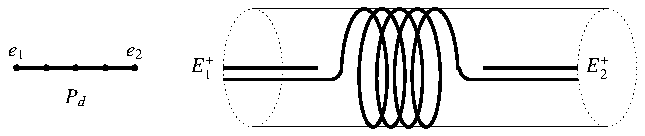
\includegraphics[width=0.90\textwidth]{figures/Fig_139_PDF245_Book233.pdf}
  \caption{一维截面上的 partially wrapped stop（原书 p.233）}
  \label{fig:partially-wrapped-stops-toric}
\end{figure}

这一方法与 Nadler、Zaslow\bookcite{195,187}提出的镜像对称中的可构造层与微局部层方法密切相关。对环簇，Bondal\bookcite{38}最先描述了可构造层方法，Fang 等人\bookcite{80,81}进一步发展。Morse 理论与微局部层之间的关系，参见 Ganatra、Pardon 与 Shende\bookcite{95}。
\end{note}

\subsection{三维情形}\label{subsec:hms-dimension-three}
为研究三维情形，需要考察环簇除子的嵌入
\[
  \iota\colon D_v=X^2_v\hookrightarrow X^3_{\boxtimes}.
\]
$X^2_v$ 上的每个线丛 $\mathcal O(d)$ 都可视为支撑在 $X^2_v$ 上的 $X^3_{\boxtimes}$ 上的层，因此是
\[
  \iota_*\mathcal O(d)\in D\mathrm{Coh}^{\bullet}_{X^2_v}(X^3_{\boxtimes})
\]
中的对象。要建立镜像对应，需要在 $Y^3_\square$ 中寻找一个以相同方式表现的对象。若计算 $D\mathrm{Coh}^{\bullet}_{X^2_v}(X^3_{\boxtimes})$ 中的自同态环，由 Serre 对偶性可知它具有 $\mathbb C\oplus\mathbb C[3]$ 的形式，这与三维球面的上同调同构。因此，一个自然想法是把拉格朗日截面 $L_d\in Y^2_\square$ 提升为 $Y^3_\square$ 中的拉格朗日球面。

前文已知，每个线丛 $\mathcal O(d)$ 对应于 $(B_v)_t$ 上方的一个拉格朗日截面 $L_d$。拓扑上，$L_d$ 是 $\mathbb C^{*2}$ 中的一张圆盘，边界落在 $W_t^{-1}(0)$ 上。三维空间 $Y^3_\square$ 可以看作 $\mathbb C^{*2}$ 上的圆锥曲线族
\[
  \{(u,v)\in\mathbb C^2\mid uv=W_t(x,y)\},
\]
而在 $W_t^{-1}(0)$ 上圆锥退化为锥。这个退化可以看作一个圆收缩为一点；所以在圆盘 $L_d$ 上方有一族圆，并在边界处收缩为点。该圆丛的全空间是一个三维球面。到目前为止我们只从拓扑角度定义了这个球面，但还可以把它实现为 $Y^3_\square$ 中的正合拉格朗日球面 $S_d$。对应关系
\[
  \iota_*\mathcal O(d)\longmapsto S_d
\]
延拓为全忠实嵌入
\[
  D\mathrm{Coh}^{\bullet}_{X^2_v}(X^3_{\boxtimes})
  \hookrightarrow D^\pi\mathrm{Fuk}^{\pm}Y^3_\square.
\]
\begin{figure}[H]\centering
  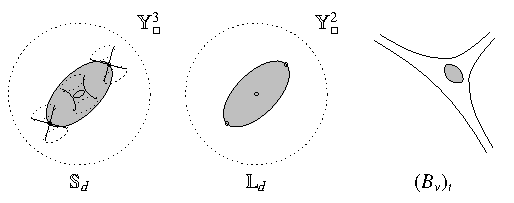
\includegraphics[width=0.73\textwidth]{figures/Fig_140_PDF246_Book234.pdf}
  \caption{三维镜像中球面与拉格朗日截面的关系（原书 p.234）}
  \label{fig:lagrangian-sphere-lift}
\end{figure}
Seidel\bookcite{219}详细研究了 Fano 情形；Abouzaid、Auroux 与 Katzarkov\bookcite{2}则将其推广到更一般的情形。

\section{远离大体积极限时}\label{sec:away-from-large-limit}
\takeaway{为得到紧流形，把曲线族紧化到环簇中并在每个柱形端放一个除子，得到 $\mathbb C[[q_1,\ldots,q_r]]$ 上的相对 Fukaya 范畴；$B$ 侧相应给势函数加入极端单项式，两侧参数由形式幂级数环的自同构联系。亏格 $2$ 曲线给出 Seidel 定理，椭圆曲线经极对偶给出反射多边形与 Batyrev 型构造。}
我们上面讨论的镜像对称例子都属于大体积极限。这里的意思是，辛形式测得的面积不起作用，因此可对 $\omega$ 重新缩放而不改变范畴。这也意味着可以在 $\mathbb C$ 上工作，而无须使用 Novikov 域。在 $B$ 侧，范畴只取决于环簇的组合结构。

大体积极限的缺点是，所考虑的辛流形必然非紧。若要研究紧辛流形，就必须通过添加额外结构来补全这些非紧版本。最直接的办法是加入除子，并考察相对 Fukaya 范畴。

先看曲线的情形。在大体积极限下，辛簇是带穿孔黎曼曲面 $Y^1_\square$，由 $W_t\colon\mathbb C^{*2}\to\mathbb C$ 的零点集确定。它是带柱形端的正合 Liouville 流形，每个穿孔对应一个端，也等价于热带曲线的一条无限腿。每条腿由 $W_t$ 的 Newton 多边形边界上的一条基本边确定。最容易想象的例子是三穿孔球面：把
\[
  X+Y+1=0\subset\mathbb C^{*2}
\]
嵌入射影平面，即可将它紧化为射影直线。
\begin{figure}[H]\centering
  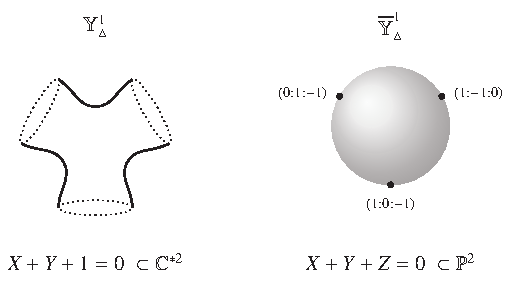
\includegraphics[width=0.64\textwidth]{figures/Fig_141_PDF247_Book235.pdf}
  \caption{三穿孔球面的射影紧化（原书 p.235）}
  \label{fig:pants-projective-compactification}
\end{figure}
一般的 $Y^1_\square$ 如何紧化？思路是把 $\mathbb C^{*2}$ 紧化为环簇 $V$，再考察 $Y^1_\square\subset\mathbb C^{*2}\subset V$ 的闭包。函数 $W_t$ 是若干单项式的线性组合，这些单项式对应 Newton 多边形 $\square$ 中的格点。我们可以把它们解释为环簇上某个线丛 $\mathcal O(d)$ 的截面；该簇的射线向量是 Newton 多边形各边的向内法向量。这个簇或其某个适当的消解，就是所需的紧化。

\begin{example}[两种环簇紧化]\label{ex:toric-compactifications}
考察以下两个例子。
\begin{enumerate}[label=(\roman*)]
  \item\label{ex:triangle-compactification} 令
  \[
    W_t=t+X+Y+X^{-1}Y^{-1}.
  \]
  其 Newton 多边形是由
  \[
    m_1=(1,0),\qquad m_2=(0,1),\qquad m_3=(-1,-1)
  \]
  张成的三角形，各边的向内法向量为
  \[
    n_1=(2,-1),\qquad n_2=(-1,2),\qquad n_3=(-1,-1).
  \]
  构造二维锥为 $\mathbb R_{\geq0}n_i+\mathbb R_{\geq0}n_j$ 的环簇 $V$。这个簇不是光滑的，但对其锥作细分可以得到消解 $\widetilde V$；补集 $\widetilde V\setminus\mathbb C^{*2}$ 由九条 $\mathbb P^1$ 组成，每条对应一条射线向量，并且这些射影直线按环状相交。
  \begin{figure}[H]\centering
    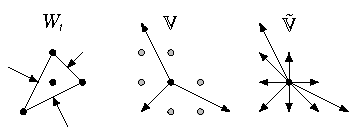
\includegraphics[width=0.48\textwidth]{figures/Fig_142_PDF247_Book235.pdf}
    \caption{三角形 Newton 多边形及其环簇消解（原书 p.235）}
    \label{fig:triangle-toric-compactification}
  \end{figure}
  函数 $W_t$ 可视为 $\mathcal O_V(1)$ 的截面，其中 $1$ 把每个射线向量 $n_i$ 映到 $1$；它也可视为 $\mathcal O_{\widetilde V}(1)$ 的截面。对通有的 $W_t$，零点集 $\overline Y^1_\square$ 与对应于 $n_i$ 的三条 $\mathbb P^1$ 各交于一点 $p_i$，但不与另外六条新增的 $\mathbb P^1$ 相交。
  \item\label{ex:projective-plane-compactification} 令
  \[
    W_t=t+X^2Y^{-1}+XY^{-1}+Y^{-1}+X^{-1}Y^{-1}
        +X^{-1}+X^{-1}Y+X^{-1}Y^2+Y+X.
  \]
  此时 Newton 多边形的三个法向方向为
  \[
    n_1=(1,0),\qquad n_2=(0,1),\qquad n_3=(-1,-1),
  \]
  相应的环簇就是光滑的 $\mathbb P^2$。该曲面有三条 $\mathbb P^1$；因为相应的方程是三次方程（等价地，热带曲线沿每条边有三条腿），$W_t^{-1}(0)$ 的紧化与每条 $\mathbb P^1$ 都交于三点。
  \begin{figure}[H]\centering
    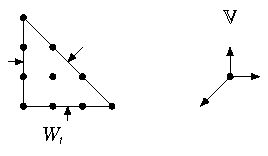
\includegraphics[width=0.53\textwidth]{figures/Fig_143_PDF248_Book236.pdf}
    \caption{第二个 Newton 多边形紧化示意（原书 p.236）}
    \label{fig:second-toric-compactification}
  \end{figure}
\end{enumerate}
\end{example}

我们可以通过加入一个除子 $D$ 来形变 wrapped Fukaya 范畴，其中 $D$ 在每个柱形端各取一点。但如例 8.21(ii) 所示，有些柱形端在紧化后会落在同一个除子上。这提示我们应给这些端使用相同的形变系数，从而得到定义在
\[
  \mathbb C[[q_1,\ldots,q_r]]
\]
上的相对 Fukaya 范畴 $\mathrm{cuFuk}^{\pm}(Y^1_\square,D)$，其中 $r$ 是 Newton 多边形边的数目。

要得到镜像对应，还需要形变 $B$ 模型。回忆一下，带穿孔黎曼曲面的镜像是 Landau--Ginzburg 模型 $(X^3_\square,\ell)$，其中整体函数 $\ell$ 是 $X^m\in\mathcal O(X^3_\square)$，且 $m=(0,0,1)\in M$。对这个 $B$ 模型，最简单的形变方法是给 $\ell$ 添加单项式项。它们必须来自结构层的整体截面：
\[
  \mathcal O(X^3_\square)
  =\mathbb C\{X^m\mid
  \text{对所有 }u\in\square,\ \langle m,(u,1)\rangle\geq0\}.
\]
这些单项式对应于对偶锥 $\sigma^\vee_\square$ 中的格点。该锥的射线向量与 $\sigma_\square$ 的面互为对偶，而这些面又与 $\square$ 的边一一对应。因此，对偶锥由形如
\[
  e_i=(n_i,c_i)
\]
的向量张成，其中 $n_i$ 是 $\square$ 某条边的向内法向量，$c_i\in\mathbb Z$ 则取决于 $\square$ 在 $\mathbb R^2$ 中的位置。这些射线向量对应的单项式称为极端单项式，可以加入势函数。首先考察 Landau--Ginzburg 模型
\[
  \mathrm{cuTw}(X^3_\square,\ell_q),
  \qquad \ell_q=\ell+\sum_iq_iX^{e_i}.
\]
这给出定义在 $\mathbb C[[q_1,\ldots,q_r]]$ 上的带曲率范畴，其中 $r$ 是多边形的边数。它恰好等于 $A$ 模型形变所用的参数数目。因此，我们预期这两种形变彼此对应，并由此在无曲率部分之间得到导出等价。当然，不能指望两侧的参数空间直接一一对应；我们预期存在形式幂级数环的一个自同构 $\alpha$，把两侧的参数互相转换。
\begin{figure}[H]\centering
  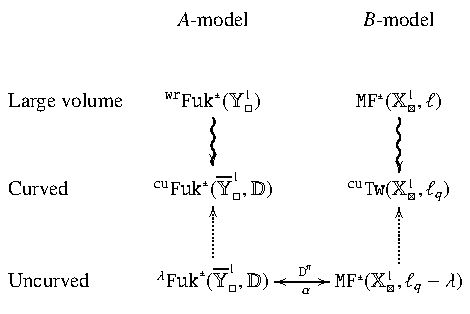
\includegraphics[width=0.82\textwidth]{figures/Fig_144_PDF249_Book237.pdf}
  \caption{$A$、$B$ 模型中的大体积极限与曲率形变（原书 p.237）}
  \label{fig:large-volume-curved-models}
\end{figure}

若在 $\overline Y^1_\square$ 上选择特定的辛形式 $\omega$，则可在 $A$ 侧对 Novikov 环上的完整 Fukaya 范畴工作。此时我们预期存在一个环同态
\[
  \beta\colon\mathbb C[[q_1,\ldots,q_r]]\to\Lambda
\]
实现参数之间的转换。这些启发式想法已在若干具体情形中得到部分验证。

\subsection*{亏格为 2 的曲线}
取环 $\mathbb C[X,Y,Z]$，并令群 $G=\langle g\mid g^5=1\rangle$ 作用为
\[
  g(x,y,z)=(\zeta x,\zeta y,\zeta^3z),
\]
其中 $\zeta$ 是五次单位根。为了求不变量，先考察 $\mathbb C[X^{\pm1},Y^{\pm1},Z^{\pm1}]^G$。此环由
\[
  U=XY^{-1},\qquad V=X^2Y^3,\qquad W=XYZ
\]
自由生成，并且
\[
  U^iV^jW^k\in\mathbb C[X,Y,Z]
  \quad\Longleftrightarrow\quad
  i+2j+k\geq0,\quad -i+3j+k\geq0,\quad k\geq0.
\]
因此，不变量环同构于由锥
\[
  \sigma=\mathbb R_{\geq0}(1,2,1)
       +\mathbb R_{\geq0}(-1,3,1)
       +\mathbb R_{\geq0}(0,0,1)
\]
张成的仿射环簇。由此
\[
  \mathbb A^3//G\cong X^3_\square,
\]
其中 $\square$ 如下图所示。
\begin{figure}[H]\centering
  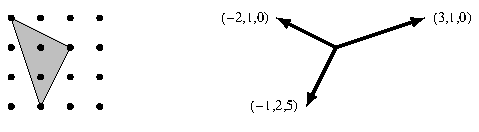
\includegraphics[width=0.62\textwidth]{figures/Fig_145_PDF249_Book237.pdf}
  \caption{亏格 2 曲线对应的 Newton 多边形（原书 p.237）}
  \label{fig:genus-two-newton-polygon}
\end{figure}

这与 Newton 多边形顶点为 $(1,2),(-1,3),(0,0)$ 的 $X^3_\square$ 相同。固定该多边形的任一三角剖分，都可以把 $X^3_{\boxtimes}$ 解释为 $\mathbb A^3//G$ 的一个消解。另一方面，$A$ 模型 $Y^1_\square$ 是一条亏格为 $2$、带三个穿孔的曲线，因为这个多边形有两个内部格点、三个边界格点。

在 $A$ 侧填上穿孔，对应于按照对偶锥的射线加入单项式：
\[
  U^3V=X^5,\qquad U^{-2}V=Y^5,\qquad
  U^{-1}V^{-2}W^5=Z^5.
\]
因此可以把势函数写为不变函数
\[
  \ell_q=XYZ+q_1X^5+q_2Y^5+q_3Z^5.
\]
在 $A$ 侧和 $B$ 侧，参数都没有出现在无穷级数中，所以镜像对应可以用普通的 $\mathbb C$-线性范畴表述。

\begin{theorem}{Seidel 的亏格二镜像定理\bookcite{220}}{seidel-genus-two-mirror}
设 $\Sigma_2$ 是一条亏格为 $2$ 的曲线，将其视为辛流形，并令 $\widetilde X$ 是 $\mathbb A^3//\mathbb Z_5$ 的一个 crepant 消解\index{crepantxiaojie@crepant 消解|hyperpage}，则有等价
\[
  D^\pi\mathrm{Fuk}^{\pm}(\Sigma_2)
  \cong_\infty D^\pi\mathrm{MF}^{\pm}
  (\widetilde X,XYZ-X^5-Y^5-Z^5).
\]
\end{theorem}
\begin{proof}[证明思路]
该定理由构造一个生成元并证明其自同态环是外代数 $\Lambda_3$ 的形变，再通过分类外代数的形变来证明这些形变彼此等价。也可以不用 $\widetilde X$，而直接在商栈 $[\mathbb A^3/\mathbb Z_5]$ 上工作。更多内容见\bookcite{220}。
\end{proof}

\begin{note}\label{note:efimov-higher-genus}
\textbf{注 8.23.} Efimov\bookcite{71}利用 $\mathbb Z_{2g+1}$ 在 $\mathbb A^3$ 上的作用，把该定理推广到了亏格 $g\geq3$ 的曲线。
\end{note}

\subsection*{椭圆曲线}
对椭圆曲线可以采取类似策略，考察 $\mathbb A^3$ 上的 $\mathbb Z_3$ 作用；此时会出现一些额外特征。首先，椭圆曲线是 Calabi--Yau 流形，因此可以把 Fukaya 范畴提升为 $\mathbb Z$-分次版本。另一方面，多项式 $\ell_q$ 是三次齐次的，所以可以考察分次矩阵分解，而非普通矩阵分解。Orlov 的结果使我们能够把分次矩阵分解范畴
\[
  \mathrm{grMF}^{\bullet}(\mathbb C[X,Y,Z],\ell_q)
\]
解释为 $\mathbb P^2$ 中 $\ell_q$ 零点集的凝聚层导出范畴；该零点集又是一条椭圆曲线 $E^\vee$。因此预期有对应
\[
  D^\pi\mathrm{Fuk}^{\bullet}(E,D)
  \cong_\infty\mathrm{grMF}^{\bullet}(\mathbb C[X,Y,Z],\ell_q)
  \cong_\infty D\mathrm{Coh}^{\bullet}E^\vee.
\]
与高亏格曲线的情形不同，$A$ 侧有无穷多个圆盘，所以形变参数会出现幂级数。

椭圆曲线的镜像仍是椭圆曲线，这一点已在许多框架下得到详细研究。Polishchuk 与 Zaslow\bookcite{205}最先描述了凝聚层导出范畴对象与 Fukaya 范畴对象之间的对应。Lekili 与 Perutz\bookcite{162,161}研究了单个除子的相对 Fukaya 范畴情形；Lekili 与 Polishchuk\bookcite{164}研究了由多个点组成的除子情形。他们从椭圆曲线的另一种表示出发。关于 $E^\vee\subset\mathbb P^2$ 及其非交换推广，参见 Cho、Hong 与 Lau 的工作\bookcite{55,154}。

\subsection*{极对偶性\index{jiduiou@极对偶|hyperpage}}
椭圆曲线的 $A$、$B$ 模型之间还存在一种引人注目的对称性。由例\ref{ex:toric-compactifications}可知，椭圆曲线 $E=Y^1_\square$ 就是例 8.21\hyperref[ex:triangle-compactification]{(i)}的紧化 $\widetilde V$ 中 $W_t$ 的零点集；而 $E^\vee$ 是 $\ell_q$ 在 $\mathbb P^2$ 中的零点集，$\mathbb P^2$ 正是该例\hyperref[ex:projective-plane-compactification]{(ii)}所用的紧化。因此，$W_t$ 与 $\ell_q$ 都在由含一个内部格点的多边形所对应的环簇中切出一条椭圆曲线。

\begin{definition}{反射多边形与极对偶多边形}{reflexive-polygon}
若 Newton 多边形 $\square$\index{fansheduobianxing@反射多边形|hyperpage} 恰有一个内部格点，且该点为 $0\in\mathbb Z^2=M$，则称 $\square$ 为反射多边形。这意味着 $\square$ 的边可写为
\[
  \langle m,u\rangle+1=0,
\]
其中 $u$ 是 $\operatorname{Hom}(M,\mathbb Z)=M^\vee=N$ 中的本原向量。由这些向量张成的凸包 $\diamond\subset N_{\mathbb R}$ 称为极对偶多边形。注意，由 $u$ 与 $m$ 的对称性可知，极对偶多边形 $\diamond$ 也仍是反射多边形。
\end{definition}

\begin{theorem}{二维反射多边形分类}{classification-reflexive-polygons}
在 $\mathrm{GL}_2(\mathbb Z)$ 变换意义下，恰有 $16$ 个反射多边形，如下图所列。其中前六列两两构成对偶对，最后两列则在某个线性变换下自对偶。
\begin{figure}[H]\centering
  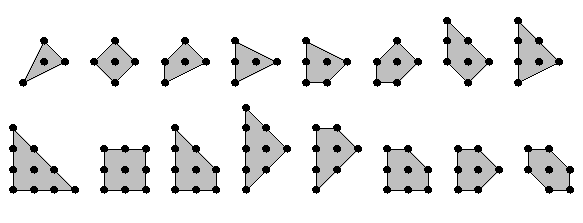
\includegraphics[width=0.82\textwidth]{figures/Fig_146_PDF251_Book239.pdf}
  \caption{二维反射多边形及其极对偶关系（原书 p.239）}
  \label{fig:sixteen-reflexive-polygons}
\end{figure}
\end{theorem}

从一个反射多边形 $\square$ 出发，把 $v=(0,0)$ 与其顶点相连，就得到一个奇异 Fano 簇的扇；再把 $v$ 连到边界上的其他格点即可消解其奇点。所得消解 $V=X^2_v$ 是弱 Fano 簇，这是 Fano 簇的轻微推广。线丛 $\mathcal O_V(1)$ 的整体截面是由极对偶多边形 $\diamond$ 中的单项式线性组合而成。取通有整体截面 $W\in\mathcal O_V(1)(V)$，其零点集是一条椭圆曲线 $E\subset V$，即一维 Calabi--Yau 簇。对极对偶多边形作同样构造，得到另一个弱 Fano 簇 $V^\vee$ 及其截面 $W^\vee$；后者的零点集是另一条椭圆曲线 $E^\vee\subset V^\vee$。对于适当的辛结构和整体截面选择，我们预期 $E$ 的 Fukaya 范畴与 $E^\vee$ 的凝聚层导出范畴等价，反向亦然。若 $\square$ 是图中第一种反射多边形，就得到上一小节描述的对应；若是第二种，则得到嵌入 $\mathbb P^1\times\mathbb P^1$ 的椭圆曲线镜像对称，详见\bookcite{154}。

这一总体思想最早由 Batyrev\bookcite{22}提出。每个 $n$ 维反射多面体都定义一个带线丛的 $n$ 维弱 Fano 簇。该线丛的通有截面给出一个 Calabi--Yau 超曲面；镜像 Calabi--Yau 簇则由极对偶多面体按同样方式构造。
% [Tutor Note: 极对偶的几何内容是“交换 Kähler 自由度与复结构自由度”：$\square$ 一侧给出弱 Fano 簇 $V$ 上的椭圆曲线 $E$，$\diamond$ 一侧给出 $V^\vee$ 上的 $E^\vee$，而 $W$ 与 $W^\vee$ 的系数分别充当对方的模参数。二维反射多边形恰有 $16$ 个，对应 $16$ 类 del Pezzo 型弱 Fano 曲面；这是 Batyrev 对偶在复二维的实例。]

这一设想已从许多角度得到研究并向多个方向推广\bookcite{24,25}。在经典镜像对称方法中，它被用于验证若干重要镜像对的 Hodge 数猜想\bookcite{22,23,56}。从同调镜像对称角度看，Seidel\bookcite{221}研究了 $\mathbb P^3$ 中的四次超曲面情形（相应反射多面体由 $\mathbb R^3$ 的标准坐标向量与 $(-1,-1,-1)$ 张成）。再高一维，$\mathbb P^4$ 中的五次超曲面是最初引出镜像对称的例子\bookcite{51}。这一情形的同调版本由 Nohara 与 Ueda\bookcite{194}证明，更一般的各维情形由 Sheridan\bookcite{223}证明。

\subsection*{Landau--Ginzburg 模型之间的镜像对称}
我们不一定只能得到两个 Calabi--Yau 簇之间的对应；也可以推广这一构造，得到两个 Landau--Ginzburg 模型之间的镜像对称。设 $a=(a_{ij})$ 是一个系数为正整数的可逆 $n\times n$ 矩阵。由 $a$ 构造多项式
\[
  W_a=\sum_iX_1^{a_{i1}}\cdots X_n^{a_{in}}
\]
和环 $R=\mathbb C[X_1,\ldots,X_n]$。$W_a$ 中的每个单项式都是环面 $T\subset\mathbb A^n=V(R)$ 上的特征。在 $T$ 中有一个固定 $W_a$ 的有限子群 $G_a$，我们取定其子群 $\Gamma\subset G_a\subset T$。

对偶一侧的多项式环为 $R^\vee=\mathbb C[Y_1,\ldots,Y_n]$，对偶多项式为
\[
  W_a^\vee=\sum_iY_1^{a_{1i}}\cdots Y_n^{a_{ni}}.
\]
固定 $W_a^\vee$ 的有限子群 $G_a^\vee$ 可自然认作 $\operatorname{Grp}(G_a,\mathbb C^*)$，并把 $\Gamma$ 的湮灭子群记作 $\Gamma^\vee$。由此得到两个带栈结构的 Landau--Ginzburg 模型
\[
  ([\mathbb A_X^n/\Gamma],W_a),
  \qquad ([\mathbb A_Y^n/\Gamma^\vee],W_a^\vee),
\]
它们应当互为镜像。与前述情形类似，一侧势函数中的每个单项式对应于另一侧仿射空间中的一个环簇除子；现在还包含额外的 orbifold 群作用，用以记录这些单项式可能是射线向量的倍数这一事实。

最简单的情形是 $n=1$ 且 $\Gamma$ 平凡；此时 $W_a=X^a$、$W_a^\vee=Y^a$，并且
\[
  D^\pi\mathrm{drFuk}^{\pm}(\mathbb C,X^a)
  \cong_\infty\mathrm{MF}^{\pm}(\mathbb C[Y]\star\mathbb Z_a,Y^a).
\]
左侧可以重新解释为 $\mathbb C$ 上带有趋向无穷远 stop 的 partially wrapped Fukaya 范畴；等价地，是边界上标有 $a$ 个点的圆盘的 Fukaya 范畴。从这个角度看，我们重新得到与第\ref{subsec:linear-quiver}节线性箭图相应的镜像对称。

这套思想也可用于尖点奇点 $(\mathbb A^2,X^3+Y^2)$ 的镜像对称（见\bookcite{161}，更一般情形见\bookcite{107}）；Ueda\bookcite{247}、Lekili\bookcite{169}等人也研究了相关对偶。此外，这些带栈结构的模型还可以与任意环簇结合使用\bookcite{59}。

\section{镜像与纤维化}\label{sec:mirrors-and-fibrations}
\takeaway{SYZ 猜想断言镜像对由互为对偶的特殊拉格朗日环面纤维化联系：$X^\vee$ 上的点层对应 $X$ 中带 $U(1)$ 局部系统的拉格朗日环面，故 $X^\vee$ 是这些环面的模空间。大体积极限下由矩映射 $\log_t$ 实现该纤维化，并由 Gross--Siebert 退化给出组合版本。}
我们已经看到，利用热带几何与环簇几何之间的对偶，可以寻找镜像对并证明一些同调镜像对称实例。从历史上看，这种解释出现得较晚。镜像对称最初只针对紧致 Calabi--Yau 流形提出，涉及计数伪全纯映射的数值不变量与镜像流形上的某些复积分之间的对偶。这些不变量的关系最初表述为生成函数之间的对应，后来才被重新解释为范畴等价。

为了描述两个镜像流形之间的关系，Strominger、Yau 与 Zaslow\bookcite{237}借助弦论中的 $T$-对偶提出一个猜想，下面将予以讨论。$T$-对偶的若干数学处理可参见\bookcite{19,77}。

\subsection{SYZ 纤维化}\label{subsec:syz-fibrations}
回忆一下，$n$ 维 Calabi--Yau Kähler 流形 $M$ 带有三种结构：复结构
\[
  J\colon TM\to TM,
\]
辛结构 $\omega\in\Omega^2M$，与复体积形式 $\Omega\in\Omega^n_{\mathbb C}M$。

\begin{definition}{特殊拉格朗日子流形与特殊拉格朗日环面纤维化}{special-lagrangian-fibration}
若拉格朗日子流形 $L\subset M$ 上的复体积形式 $e^{-i\theta}\Omega$ 限制为实体积形式，则称 $L$ 为相位 $\theta$ 的特殊拉格朗日子流形\index{teshulagelangriziliuxing@特殊拉格朗日子流形|hyperpage}。若映射 $\pi\colon M\to B$ 的每个纤维都是具有相同相位的特殊拉格朗日环面，则称 $\pi$ 为特殊拉格朗日环面纤维化\index{teshulagelangrihuanmianxianweihua@特殊拉格朗日环面纤维化|hyperpage}。
\end{definition}

\begin{example}[椭圆曲线的特殊拉格朗日纤维化]
考虑复流形
\[
  M=\mathbb C/(\mathbb Z+i\mathbb Z),
\]
配备辛形式 $\omega=dx\wedge dy$，其中 $z=x+iy$ 是 $\mathbb C$ 上的标准坐标。取复体积形式 $\Omega=dz$。这个一维紧致 Calabi--Yau 流形有一个显然的特殊拉格朗日环面纤维化，其底空间为 $B=\mathbb R/\mathbb Z$：
\[
  \pi\colon M\to B,\qquad x+iy\longmapsto y.
\]
该映射的纤维是水平圆周，所以纤维化的相位为 $0$。若改为投影到 $x$ 坐标，则得到相位为 $\pi/2$ 的纤维化。更一般地，对每个
\[
  A=\begin{pmatrix}a&c\\b&d\end{pmatrix}\in\mathrm{GL}(2,\mathbb Z),
\]
映射 $\pi\circ A^{-1}$ 都给出一个相位为 $\arg(a+bi)$ 的特殊拉格朗日环面纤维化。
\end{example}

还可以用另一种方式看这个例子。考察圆周 $S^1$ 及其余切丛 $T^*S^1$。该余切丛是平凡向量丛，因此可以在每个纤维 $T_p^*S^1$ 中选取一个格 $\Lambda_p^*\subset T_p^*S^1$。余切丛有自然辛结构，该结构自然下降到商丛
\[
  M=T^*S^1/\Lambda^*.
\]
特殊拉格朗日子流形恰好是纤维
\[
  L_p=T_p^*S^1/\Lambda_p^*.
\]
另一方面，切丛 $TS^1$ 带有自然复结构，而格 $\Lambda_p^*\subset T_p^*S^1$ 确定一个对偶格 $\Lambda_p\subset T_pS^1$。向量空间 $V$ 中一个格的对偶格由所有把该格映到 $\mathbb Z$ 的协向量组成。若该格有一组基，则其对偶格由对偶基生成。对偶格取商便得到实环面
\[
  M^\vee=TS^1/\Lambda,
\]
和配对
\[
  \langle\ ,\ \rangle_p\colon
  T_p^*S^1/\Lambda_p^*\times T_pS^1/\Lambda_p
  \longrightarrow\mathbb R/\mathbb Z\cong U(1).
\]
整体上，这给出如下图表，其中纤维两两对偶：
\begin{figure}[H]\centering
  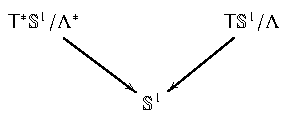
\includegraphics[width=0.43\textwidth]{figures/Fig_147_PDF255_Book243.pdf}
  \caption{余切环面与切环面的对偶纤维（原书 p.243）}
  \label{fig:cotangent-torus-duality}
\end{figure}
\begin{figure}[H]\centering
  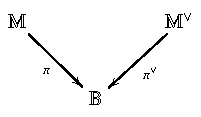
\includegraphics[width=0.38\textwidth]{figures/Fig_148_PDF255_Book243.pdf}
  \caption{两对偶环面纤维化在共同底空间上的对应（原书 p.243）}
  \label{fig:dual-torus-fibrations}
\end{figure}

由于 $M$ 与 $M^\vee$ 构成镜像对，这提示镜像流形应当由互为对偶的拉格朗日纤维化联系起来。一般而言，紧致 Calabi--Yau 流形上的特殊拉格朗日环面纤维化很难找到\bookcite{102,101,103}；多数情形下，除非放宽对 $\pi$ 的要求，否则它们并不存在。首先，不应要求底空间 $B$ 是光滑流形；其次，也不应要求每个纤维都是特殊拉格朗日环面，只要求通有纤维如此\bookcite{129}。也就是说，只有在 $B$ 的一个稠密开子集上，纤维才是互为对偶的特殊拉格朗日环面。特殊拉格朗日纤维化的背景可参阅 Hitchin\bookcite{113} 与 Joyce\bookcite{128} 的讲义。

\begin{conjecture}{Strominger--Yau--Zaslow\bookcite{237}}{syz-conjecture}
若两个 Calabi--Yau 流形 $(M,M^\vee)$ 互为镜像，则存在一个底空间 $B$ 及映射 $\pi,\pi^\vee$，使图表
\[
\begin{array}{ccc}
  M & \xrightarrow{\,\pi\,} & B \\[-2pt]
  M^\vee & \xrightarrow{\,\pi^\vee\,} & B
\end{array}
\]
所表示的 $\pi\colon M\to B$ 与 $\pi^\vee\colon M^\vee\to B$ 都是（可能奇异的）特殊拉格朗日环面纤维化；并且对一般点 $b\in B$，存在配对
\[
  \langle\ ,\ \rangle_b\colon
  \pi^{-1}(b)\times(\pi^\vee)^{-1}(b)\to U(1).
\]
\end{conjecture}

这个猜想与同调镜像对称有何关系？回忆一下，完整 Fukaya 范畴中我们关注的对象是带 $U(1)$ 局部系统的拉格朗日子流形（见注~\ref{note:unitary-local-systems}）。若 $X$ 与 $X^\vee$ 互为镜像，则有等价
\[
  D^\pi\mathrm{Fuk}(X)\cong D^\pi\mathrm{Coh}(X^\vee).
\]
$X^\vee$ 上的点层是 $D^\pi\mathrm{Coh}(X^\vee)$ 中的对象，其自同态代数是外代数。粗略来说，拉格朗日子流形 $L$ 的自同态代数等于它的上同调环；因此我们预期，点层会对应于带局部 $U(1)$-系统的拉格朗日环面。

这表明，一般而言，$X^\vee$ 上点层的模空间应当参数化 $X$ 上带 $U(1)$-局部系统的平行拉格朗日环面。对每个拉格朗日环面，可选的 $U(1)$-局部系统本身构成一个实 $n$ 维环面。因此，$X^\vee$ 一般由若干个实 $n$ 维环面组成；同一个拉格朗日环面对应的点层位于同一个这样的环面中。把这些环面取商，便得到某个 $n$ 维空间 $B$ 及映射 $\pi^\vee\colon X^\vee\to B$。

位于不同点的两个点层之间没有态射，这类似于两个不相交拉格朗日子流形之间的 Hom 空间为零。这提示 $B$ 中不同点对应的拉格朗日环面彼此不相交；这族 $n$ 维环面一般会铺满 $2n$ 维空间 $X$，从而得到投影 $\pi\colon X\to B$。纤维
\[
  L_b=\pi^{-1}(b)
\]
是一个环面，可写作 $\mathbb R^n/\Lambda$，其中格 $\Lambda\cong\pi_1(L_b)$。$L_b$ 上的 $U(1)$ 局部系统空间自然同构于对偶环面：
\[
  \operatorname{Hom}(\Lambda,U(1))
  \cong\operatorname{Hom}(\Lambda,\mathbb R/\mathbb Z)
  \cong\frac{\operatorname{Hom}(\Lambda,\mathbb R)}
  {\operatorname{Hom}(\Lambda,\mathbb Z)}
  \cong\frac{\mathbb R^n}{\Lambda^*}.
\]
% [Tutor Note: 第二处同构用了 $\Lambda\cong\mathbb Z^n$：逐个生成元提升即可看出 $\operatorname{Hom}(\Lambda,\mathbb R)\to\operatorname{Hom}(\Lambda,\mathbb R/\mathbb Z)$ 满射，其核正是 $\operatorname{Hom}(\Lambda,\mathbb Z)$。最后一步把 $\Lambda$ 换成对偶格 $\Lambda^*=\operatorname{Hom}(\Lambda,\mathbb Z)$；若改变 $\Lambda$ 与 $\pi_1(L_b)$ 的同一化，$B$ 的坐标会差一个 $\mathrm{GL}(n,\mathbb Z)$ 变换，这正是镜像构造中的整变换不确定性。]
这番推理并非证明，却说明了在一定条件下 SYZ 猜想成立的缘由。另一种观点见\bookcite{245}。

SYZ 猜想为镜像对的存在提供了漂亮的几何解释，但它既不容易证明，也不清楚是否在完全一般的情形下成立\bookcite{130}。一个原因是，特殊拉格朗日子流形通常很难构造，更不用说构造几乎覆盖整个空间的一族此类子流形。此外，纤维化的底空间通常是奇异的；如何构造这个底空间、它应满足哪些性质，都还不清楚。

\subsection*{极限情形}
为绕开这些困难，最好考察大体积极限等极限情形。此时可以利用环簇几何与热带几何之间的对偶。复环面有一个自然的拉格朗日环面纤维化
\[
  \log_t\colon T\to\mathbb R^n.
\]
若 $V$ 是一个环簇，其射线向量垂直于多面体 $\square$ 的各边，则可用矩映射 $\mu\colon V\to\square$ 延拓这个纤维化，使 $T$ 映到 $\square$ 的内部，而每个射线向量对应的除子映到相应的面\bookcite{89}。

现在设
\[
  W_t=1+tf,
\]
其中 $f$ 是 Newton 多面体为反射多面体 $\square$ 的通有函数。纤维 $W_t^{-1}(0)\subset\mathbb C^{*n}$ 可紧化为一族 $\overline Y_t\subset V$。当 $t\ne0$ 时，映射 $\mu|_{\overline Y_t}$ 不是拉格朗日环面纤维化；但在极限 $t\to0$ 时，它变为这样的纤维化，此时族退化为
\[
  \overline Y_0=\widetilde V\setminus\mathbb C^{*n},
\]
即若干环簇的并。每个多边形的面对应一个环簇；两个面相交时，对应的环簇也相交。另一方面，极对偶多边形给出第二族 $\overline Y^\vee_t$，可视为第一族的镜像。其极限同样是若干环簇的并，但由于极对偶性，它的交复形与第一族的交复形互为对偶。

\begin{example}[椭圆曲线退化与极对偶]
从顶点为 $(\pm1,\pm1)$ 的正方形出发，可得到 $\mathbb P^1\times\mathbb P^1$ 中一族退化为四条 $\mathbb P^1$ 的椭圆曲线。每条曲线与四条 $\mathbb P^1$ 共交于八个点，每条 $\mathbb P^1$ 上有两个，位置由 $f$ 的零点决定。

极对偶是顶点为 $(\pm1,0),(0,\pm1)$ 的正方形。它给出另一族椭圆曲线，位于有四个二阶商奇点的环簇中，每个顶点对应一个奇点。该族退化为四条在这些二阶奇点处相交的 $\mathbb P^1$。每条曲线与四条 $\mathbb P^1$ 各交于一点，位置由 $f$ 的零点决定。
\begin{figure}[H]\centering
  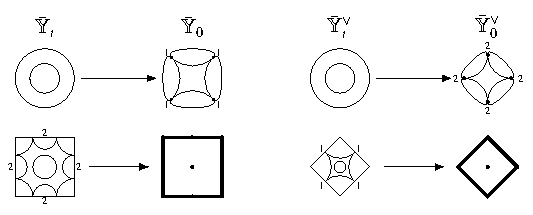
\includegraphics[width=0.96\textwidth]{figures/Fig_149_PDF257_Book245.pdf}
  \caption{例 8.29 中的对偶退化（原书 p.245）}
  \label{fig:elliptic-degeneration-polar-dual}
\end{figure}
\end{example}

这一思想在 Gross--Siebert 研究纲领中得到进一步发展与推广。其基本目标是通过一族簇研究镜像对称，这些簇退化为若干环簇之并，相邻的环簇沿轨道层相交。退化的交复形连同一些附加数据，可以通过离散 Legendre 变换重构镜像族。该方法使用代数几何、仿射结构、对数几何和热带几何中的许多技巧。关于这一纲领的更多内容，参见\bookcite{104,105,250}。

\section{练习}\label{sec:chapter-eight-exercises}

\begin{exercise}\label{exer:toric-line-bundle-cohomology}
设 $v_1,\ldots,v_4$ 是 $N=\mathbb Z^2$ 中的本原向量，它们把平面分为四个凸锥
\[
  \mathbb R_{\geq0}v_i+\mathbb R_{\geq0}v_{i+1}
\]
（下标按循环理解），并令 $\Delta$ 为对应的扇。对每个 $d\in\mathbb Z^4$，可在 $X_\Delta$ 上定义线丛 $\mathcal O(d)$。其 Čech 复形可按 $M=N^\vee$ 分次。请用几何方式，根据 $v_i,d_i$ 计算次数 $m\in M$ 部分的层上同调。
\end{exercise}

\begin{exercise}\label{exer:five-line-bundle-tilting}
设 $X$ 是由下图环簇图确定的完备环簇。
\begin{figure}[H]\centering
  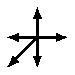
\includegraphics[width=0.17\textwidth]{figures/Fig_150_PDF258_Book246.pdf}
  \caption{练习 8.2 中的环簇图（原书 p.246）}
  \label{fig:exercise-eight-two-fan}
\end{figure}
说明为什么可以把 $X$ 看成在两个点处爆破的射影平面，或在一个点处爆破的 $\mathbb P^1\times\mathbb P^1$。找一个由五个形如 $\mathcal O(d)$ 的线丛直和组成的倾斜丛。
\end{exercise}

\begin{exercise}\label{exer:isolated-toric-singularity}
设 $v_1,\ldots,v_k\in\mathbb Z^2\times\{1\}$ 是位于高度 $1$ 的凸格点多边形 $\square$ 的顶点，令 $X^3_\square$ 是由锥
\[
  \sum_i\mathbb R_{\geq0}v_i
\]
对应的环簇。证明：$X^3_\square$ 有孤立奇点，当且仅当边上没有额外格点，且 $\square$ 不是基本三角形。
\end{exercise}

\begin{exercise}\label{exer:pick-theorem}
证明 Pick 定理：格点多边形的面积为
\[
  I+\frac{B}{2}-1,
\]
其中 $I$ 是内部格点数，$B$ 是边界格点数。
\end{exercise}

\begin{exercise}\label{exer:cyclic-quotient-toric-triangle}
固定 $(a,b)\in\mathbb Z^2$，令 $G=\langle g\mid g^n=1\rangle\cong\mathbb Z/n\mathbb Z$ 在 $\mathbb C^3$ 上的作用为
\[
  g(x,y,z)=\bigl(e^{2a\pi i/n}x,
  e^{2b\pi i/n}y,e^{-2(a+b)\pi i/n}z\bigr).
\]
证明该商可以描述为环簇 $X^3_\square$，其中 $\square$ 是面积为 $n/2$ 的三角形。
\end{exercise}

\begin{exercise}\label{exer:elliptic-tropicalization}
设椭圆曲线 $E$ 的方程为
\[
  Y^2=X^3+t^aX+t^b.
\]
描述其热带化如何随 $a,b\in\mathbb Z$ 变化。
\end{exercise}

\begin{exercise}\label{exer:one-polytope-three-dimensions}
第\ref{sec:one-two-three-mirror-symmetry}节为格点多边形在维数 $1,2,3$ 中构造了镜像。类似地，$n$ 维格点多面体也可在 $n-1,n,n+1$ 维中构造镜像。现在取 $n=1$。一维格点多面体就是长度为 $k$ 的线段 $L$，可将它放在 $\mathbb Z^2$ 中高度为 $1$ 的位置。
\begin{enumerate}[label=(\roman*)]
  \item 证明
  \[
    X^{n+1}_\square\cong V\bigl(\mathbb C[X,Y,Z]/(XY-Z^k)\bigr).
  \]
  描述消解 $X^{n+1}_{\boxtimes}\to X^{n+1}_\square$ 的例外纤维。
  \item $(n-1)$ 维镜像对应预言等价
  \[
    D^\pi\mathrm{MF}^{\pm}(X^{n+1}_{\boxtimes},\ell)
    \cong_\infty D^\pi_{\mathrm{wr}}\mathrm{Fuk}^{\pm}Y^{n-1}_\square.
  \]
  若把一点的 wrapped Fukaya 范畴解释为 $\mathrm{vect}^{\pm}_{\mathbb C}$，证明此对应成立。
  \item 对 $n$ 维版本，假设 $L$ 有一个内部格点。证明这会给出 $\mathbb P^1$ 的导出范畴与一个有向 Fukaya 范畴之间的镜像对应，并给出证明策略。
  \item 对 $(n+1)$ 维版本，描述支撑在 $\mathbb P^1$ 上的 $X^{n+1}_{\boxtimes}$ 上的层导出范畴。证明它与代数
  \[
    \mathbb C[[X,Y]]\star\mathbb Z_2
  \]
  的有限维模导出范畴等价，其中 $\mathbb Z_2$ 对 $X,Y$ 都按符号作用。
\end{enumerate}
\end{exercise}

\begin{exercise}\label{exer:genus-g-toric-triangle}
调整亏格为 $g$ 的曲线的镜像构造，使它适用于任意一个内部有 $g$ 个格点、边界上没有格点的格点三角形。
\begin{enumerate}[label=(\roman*)]
  \item 证明：当 $g=2$ 时，这种构造总是给出 Seidel 的同一构造。
  \item 证明：当 $g=3$ 时，存在不止一种可能（即在格的自同构意义下有不同的三角形）。哪一种对应 Efimov 的构造？
  \item 详细研究一个 $g=3$、但不对应 Efimov 构造的三角形。描述群作用，并确定商奇点的不同可能消解。
\end{enumerate}
\end{exercise}

\begin{exercise}\label{exer:batyrev-elliptic-curve-p1-p1}
用齐次坐标 $((X:Y),(U:V))$ 描述空间 $\mathbb P^1\times\mathbb P^1$。证明：对通有的 $q$，方程
\[
  XYUV+q(X^2+Y^2)(U^2+V^2)=0
\]
的零点集是一条椭圆曲线。用 Batyrev 对偶的观点解释这一构造。
\end{exercise}

\begin{exercise}\label{exer:lg-lg-an-singularity}
为简单奇点 Landau--Ginzburg 模型
\[
  X=(\mathbb A^n,X_1^2+\cdots+X_n^2)
\]
构造 Landau--Ginzburg 镜像 $Y$，并双向证明镜像对称：$X$ 的 $A$ 模型等价于 $Y$ 的 $B$ 模型，反过来也成立。
\end{exercise}

\chapterreview{%
\textbf{全章地位。}前七章分别造出 $A$ 侧与 $B$ 侧的范畴，本章第一次把它们真正对上。作者没有直接处理紧致 Calabi--Yau 流形，而是从 $(\mathbb C^*)^n$ 与 $T^*(S^1)^n$ 这对最简单的镜像出发，逐步加入环簇与热带几何，最后把一、二、三维的构造统一成“Newton 多边形 $+$ 三角剖分”这组组合数据。后半转向 SYZ 猜想与 Gross--Siebert 纲领。

\textbf{知识脉络。}线索是“一个例子、两种几何、三个维数、一个猜想”。§8.1 用复环面把 wrapped、正合、$\mathbb Z_2$ 分次三种 Fukaya 范畴分别对应凝聚层、挠层与矩阵分解；§8.2 引入环簇，把“锥 $-$ 轨道 $-$ 除子”的字典翻译成“势函数单项式”；§8.3 用热带几何把 $t\to\infty$ 的阿米巴极限化为 Newton 多边形的对偶三角剖分；§8.4 陈述一、二、三维的镜像等价；§8.5 讨论离开大体积极限后如何紧化、加除子并加入极端单项式；§8.6 用 SYZ 纤维化解释镜像对的整体几何。

\textbf{核心结论。}（1）$D^\infty\mathrm{wrFuk}^{\bullet}(T^*(S^1)^n)\cong D\mathrm{Coh}^{\bullet}(\mathbb C^*)^n$，正合版本对应挠层，$\mathbb Z_2$ 分次版本对应 $\mathrm{MF}^{\pm}(\mathbb C^{n+2},(X_0\cdots X_n-1)Z)$；镜像上的点对应底环面 $(S^1)^n$ 上的一维局部系统，故镜像是作为对偶群出现的 $T^\vee=\operatorname{Grp}(N,\mathbb C^*)$。（2）环簇中锥与轨道一一对应，$\dim\sigma=n-\dim O_\sigma$；一维锥给出射线向量 $v_\sigma$ 与环簇除子 $D_\sigma$，$A$ 侧加入 $D_\sigma$ 恰使 $B$ 侧势函数多出单项式 $y^{v_\sigma}$，即 $W_\hbar=\sum\hbar\,y^{v_\sigma}$。（3）热带极限把几何变成组合：$W_t^{-1}(0)$ 的亏格等于 Newton 多边形的内部格点数，穿孔数等于边界格点数，三角剖分与热带曲线对偶。（4）三维对应有三条：$D^\pi\mathrm{MF}^{\pm}X^1_{\boxtimes}\simeq D^\pi\mathrm{wrFuk}^{\pm}Y^1_\square$；$D\mathrm{Coh}^{\bullet}X^2_v\hookrightarrow D^\pi\mathrm{drFuk}^{\bullet}Y^2_\square$；$D\mathrm{Coh}^{\bullet}_{X^2_v}(X^3_{\boxtimes})\hookrightarrow D^\pi\mathrm{exFuk}^{\bullet}Y^3_\square$，其中第二条在内部格点唯一（$X^2_v=\ell^{-1}(0)$）时升级为等价。

\textbf{辨析与提醒。}其一，“环簇”不是“环面”：环簇是含稠密复环面开轨道、由扇组合定义的正规簇，复环面只是它的一个开子集；“环簇除子”专指余维 $1$ 轨道闭包。其二，几种 Fukaya 范畴不要混：wrapped 用于非紧余切丛，正合用于紧正合拉格朗日，有向用于 LG 模型的盘，相对版本 $\mathrm{cuFuk}$ 用于带除子的流形，partially wrapped 则带 stop。其三，$t\to\infty$ 的热带极限与 $\hbar\to0$ 是同一退化的两种说法，阿米巴“收敛到”热带曲线是 Hausdorff 意义下的收敛，不能当作相等。其四，大体积极限丢掉紧致性与 Kähler 模：恢复紧致须紧化并加除子，所得范畴定义在 $\mathbb C[[q_1,\ldots,q_r]]$ 上，两侧参数只由形式幂级数环的自同构联系，不要指望逐一对应。

\textbf{评注。}作者的策略是用环簇与热带几何绕开一般 Calabi--Yau 流形上难以构造的特殊拉格朗日纤维化，把镜像对称化归为多边形与三角剖分的组合游戏。代价是结论基本停留在大体积极限与非紧流形，真正紧的情形只剩 SYZ 猜想与 Gross--Siebert 纲领的入口。三维部分的拆法值得注意：$B$ 侧分成 $X^1_{\boxtimes}$、$X^2_v$、$X^3_{\boxtimes}$ 三层，分别对应矩阵分解、凝聚层与支撑层，看似重复，实则正是 Abouzaid 等人“先找分裂生成元、再比自同态代数”的证明路线；三行对应当读成一个构造的三层，而非三个独立定理。椭圆曲线与极对偶两小节把 Batyrev 对偶放进同调框架，是连接经典镜像对称与范畴版本的桥梁，也是本章最值得细读之处。}
